\documentclass[a4paper]{article}
\usepackage{vntex}
%\usepackage[english,vietnam]{babel}
%\usepackage[utf8]{inputenc}

%\usepackage[utf8]{inputenc}
%\usepackage[francais]{babel}
\usepackage{a4wide,amssymb,epsfig,latexsym,multicol,array,hhline,fancyhdr}
\usepackage{amsmath}
\usepackage{lastpage}
\usepackage{float}
\usepackage[lined,boxed,commentsnumbered]{algorithm2e}
\usepackage{enumerate}
\usepackage{color}
\usepackage{graphicx}							% Standard graphics package
\usepackage{array}
\usepackage{tabularx, caption}
\usepackage{multirow}
\usepackage{multicol}
\usepackage{rotating}
\usepackage{graphics}
\usepackage{geometry}
\usepackage{setspace}
\usepackage{epsfig}
\usepackage{tikz}
\usepackage{cite}
\usetikzlibrary{arrows,snakes,backgrounds}
\usepackage{hyperref}


\hypersetup{urlcolor=blue,linkcolor=black,citecolor=black,colorlinks=true} 
%\usepackage{pstcol} 								% PSTricks with the standard color package

\newtheorem{theorem}{{\bf Định lý}}
\newtheorem{property}{{\bf Tính chất}}
\newtheorem{proposition}{{\bf Mệnh đề}}
\newtheorem{corollary}[proposition]{{\bf Hệ quả}}
\newtheorem{lemma}[proposition]{{\bf Bổ đề}}


%\usepackage{fancyhdr}
\setlength{\headheight}{40pt}
\pagestyle{fancy}
\fancyhead{} % clear all header fields
\fancyhead[L]{
 \begin{tabular}{rl}
    \begin{picture}(25,15)(0,0)
    \put(0,-8){
\includegraphics[width=8mm, height=8mm]{hcmut.png}}
    %\put(0,-8){\epsfig{width=10mm,figure=hcmut.eps}}
   \end{picture}&
	%
\includegraphics[width=8mm, height=8mm]{hcmut.png} & %
	\begin{tabular}{l}
		\textbf{\bf \ttfamily Trường Đại Học Bách Khoa Tp.Hồ Chí Minh}\\
		\textbf{\bf \ttfamily Khoa Khoa Học và Kỹ Thuật Máy Tính}
	\end{tabular} 	
 \end{tabular}
}
\fancyhead[R]{
	\begin{tabular}{l}
		\tiny \bf \\
		\tiny \bf 
	\end{tabular}  }
\fancyfoot{} % clear all footer fields
\fancyfoot[L]{\scriptsize \ttfamily Bài tập lớn môn Mạng máy tính - Niên khóa 2019-2020}
\fancyfoot[R]{\scriptsize \ttfamily Trang {\thepage}/\pageref{LastPage}}
\renewcommand{\headrulewidth}{0.3pt}
\renewcommand{\footrulewidth}{0.3pt}


%%%
\setcounter{secnumdepth}{4}
\setcounter{tocdepth}{3}
\makeatletter
\newcounter {subsubsubsection}[subsubsection]
\renewcommand\thesubsubsubsection{\thesubsubsection .\@alph\c@subsubsubsection}
\newcommand\subsubsubsection{\@startsection{subsubsubsection}{4}{\z@}%
                                     {-3.25ex\@plus -1ex \@minus -.2ex}%
                                     {1.5ex \@plus .2ex}%
                                     {\normalfont\normalsize\bfseries}}
\newcommand*\l@subsubsubsection{\@dottedtocline{3}{10.0em}{4.1em}}
\newcommand*{\subsubsubsectionmark}[1]{}
\makeatother


\begin{document}

\begin{titlepage}
\begin{center}
ĐẠI HỌC QUỐC GIA THÀNH PHỐ HỒ CHÍ MINH \\
TRƯỜNG ĐẠI HỌC BÁCH KHOA \\
KHOA KHOA HỌC - KỸ THUẬT MÁY TÍNH 
\end{center}

\vspace{1cm}

\begin{figure}[h!]
\begin{center}

\includegraphics[width=3cm]{hcmut.png}
\end{center}
\end{figure}

\vspace{1cm}


\begin{center}
\begin{tabular}{c}
\multicolumn{1}{l}{\textbf{{\Large Mạng máy tính}}}\\
~~\\
\hline

\\
\multicolumn{1}{l}{\textbf{{\Large Bài tập lớn số 1}}}\\
\\
\textbf{{\Huge Xây dựng web chat client TCP/IP}}\\
\\
\hline
\end{tabular}
\end{center}

\vspace{3cm}

\begin{table}[h]
\begin{tabular}{rrl}
%\hspace{5 cm} & GVHD: & Họ và tên\\
& & Nguyễn Quang Đức - 1810118 \\
\end{tabular}
\end{table}

\begin{center}
{\footnotesize TP. HỒ CHÍ MINH, THÁNG 10/2019}
\end{center}
\end{titlepage}


%\thispagestyle{empty}

\newpage
\tableofcontents
\newpage
%%%%%%%%%%%%%%%%%%%%%%%%%%%%%%%%%
\section{Giới thiệu ứng dụng chat}
	Ứng dụng chat này được xây dựng trên nền tảng ứng dụng web thuần túy với nhiều ưu điểm như đa nền tảng, gọn nhẹ, giao diện trực quan dễ sử dụng. Ứng dụng này được hiện thực trên nền backend là Python 3, sử dụng giao thức HTTP và SocketIO để truyền và nhận dữ liệu. Về phía client, trang web được viết bằng HTML + CSS + Javascipt với giao diện đơn giản, tối ưu cho việc chat.
	
\section{Chức năng cơ bản của ứng dụng}
	\subsection{Đăng ký người dùng}
		\begin{itemize}
			\item Giao thức sử dụng: HTTP
			\item Truy cập trang web: HTTP GET
			\item Gửi thông tin đăng ký: HTTP POST
		\end{itemize}
	
	Người dùng truy cập vào trang đăng ký tài khoản, nhập đầy đủ thông tin và bấm đăng ký. Sau đó thông tin được gửi lên server xử lý, kiểm tra và trả về kết quả. Nếu đăng ký thành công, tự động chuyển hướng đến trang cá nhân. Ngược lại, server sẽ thông báo không thể tạo tài khoản.
	
	\subsection{Gửi và nhận tin nhắn}
	\begin{itemize}
		\item Giao thức sử dụng: SocketIO
	\end{itemize}
	
	Khi người dùng nhập tin nhắn và gửi đi, tin nhắn của người dùng sẽ được gửi đến server chính. Sau đó server chính định danh các máy nhận và gửi tin nhắn trả về.\linebreak
	Tại server chính, tin nhắn của người dùng sẽ được lưu lại trong database.
	
	\subsection{Gửi và nhận file}
		\begin{itemize}
			\item Giao thức sử dụng: HTTP
			\item Gửi file: HTTP POST
			\item Nhận file: HTTP GET
		\end{itemize}
		
	Người dùng chọn file và bấm gửi file, file sẽ được trực tiếp upload lên server. Tại server sau khi nhận file sẽ gửi tin nhắn trả về tất cả thành viên trong nhóm là đường link đến file đó.\linebreak
	Để tải file về, người dùng nhấp vào tên file và và file sẽ được tải xuống.
	
	\subsection{Xem trạng thái của thành viên khác}
		\begin{itemize}
			\item Giao thức sử dụng: SocketIO
		\end{itemize}
		
	Thông tin thành viên trong nhóm sẽ được cập nhật liên tục khi có người online hoặc offline đến từng người trong nhóm.
	
\section{Chức năng nâng cao của ứng dụng}
	\subsection{Quản lý tài khoản cá nhân}
		\subsection{Đăng ký}
		Khi đăng ký tài khoản, ứng dụng yêu cầu nhập đúng định dạng email, email và tên tài khoản phải là duy nhất và xác thực password phải khớp với nhau thì mới đăng ký thành công.\linebreak
		Thông tin đăng ký của người dùng sẽ được lưu xuống database trên server chính.\linebreak
		Khi lưu các thông tin, password sẽ được mã hóa nhằm đảm bảo tính bảo mật.
		
		\subsubsection{Đăng nhập | Đăng xuất}
		Để đăng nhập vào tài khoản, người dùng bắt buộc phải nhập đúng tên tài khoản và mật khẩu đã đăng ký thì mới được cấp phép vào trang cá nhân.\linebreak
		Khi đăng xuất, người dùng sẽ được chuyển hướng về trang đăng nhập.
		
		\subsubsection{Quên mật khẩu}
		Khi người dùng không nhớ mật khẩu, có thể lấy lại mật khẩu bằng cách nhập email đã đăng ký. Vì email là duy nhất nên nếu email nằm trong danh sách người dùng đã đăng ký thì thông tin người dùng sẽ được đưa vào hàng đợi quên mật khẩu. Ngược lại, người dùng sẽ không thể lấy lại mật khẩu.\linebreak
		Sau khi gửi yêu cầu quên mật khẩu, người dùng sẽ được chuyển hướng về trang đăng nhập.\linebreak
		Người dùng phải trong trạng thái offline thì mới vào trang quên mật khẩu được.
		
		\subsubsection{Thay đổi mật khẩu}
		Người dùng sau khi đăng nhập vào hệ thống sẽ có quyền thay đổi mật khẩu. Người dùng phải nhập đúng mật khẩu cũ và xác nhận mật khẩu mới thì mới có thể thay đổi mật khẩu.
		
		\subsubsection{Trạng thái online/offline}
		Sau khi người dùng đăng nhập vào hệ thống, trạng thái của người dùng luôn được gán là online.\linebreak
		Trạng thái người dùng sẽ chuyển sang offline khi người dùng đăng xuất hoặc ngắt kết nối.
		
	\subsection{Quản lý phòng chat}
		\subsubsection{Tạo phòng chat}
		Sau khi đăng nhập, người đùng có thể tạo phòng chat theo ý muốn. Để tạo phòng chat, người dùng chỉ cần nhập tên phòng. Các phòng chat có thể trùng tên.\linebreak
		Khi tạo phòng chat thành công, phòng chat sẽ hiển thị trên trang cá nhân của người dùng.
		
		\subsubsection{Thêm người vào phòng chat}
		Khi tạo phòng chat, người dùng có thể thêm bạn bè vào phòng chat bằng cách gõ tên người dùng của bạn bè vào.\linebreak
		Server sẽ kiểm tra tên người dùng đã nhập vào và chỉ thêm người dùng vào phòng chat khi người đó có trong database của server.\linebreak
		Sau khi thêm người dùng, phòng chat sẽ được cập nhật đến tất cả thành viên có trong phòng.
		
	\subsection{Quản lý tin nhắn và file}
\section{Thiết kế ứng dụng}
	\subsection{Luồng chính}
		Bao gồm các hiện thực các giao thức HTTP và SocketIO trên server.
		
	\subsection{Quản lý người dùng}
		Bao gồm các chức năng thao tác với database liên quan đến quản lý tài khoản người dùng. 
		
	\subsection{Quản lý chat}
		Bao gồm các chức năng liên quan đến lưu trữ và tải tin nhắn
		
\section{Kết quả hiện thực}
	\subsection{Ưu điểm}
		\begin{itemize}
			\item Ứng dụng chạy nhanh và ổn định
			\item Giao diện trực quan, dễ sử dụng
			\item Có đầy đủ các tính năng cơ bản về quản lý tài khoản và quản lý chat
		\end{itemize}
		
	\subsection{Khuyết điểm}
		\begin{itemize}
			\item Nhiều chức năng vẫn chưa hiện thực kịp dù đã có trên giao diện
			\item Chưa mã hóa tin nhán, mã hóa đường dẫn lưu dữ liệu nên có thể xảy ra các vấn đề liên quan đến bảo mật
		\end{itemize}
		
\section{Hướng dẫn sử dụng ứng dụng}
	\subsection{Đăng ký tài khoản}
	Ứng dụng cho phép người dùng đăng ký tài khoản. Các thông tin của một tài khoản bao gồm:\linebreak
	\begin{itemize}
		\item Tên đầy đủ
		\item Tên người dùng
		\item Email
		\item Mật khẩu
	\end{itemize}
	Điều kiện bắt buộc là tên người dùng và email phải là duy nhất.\linebreak
	Nếu tất cả thông tin chính xác, thì sau khi đăng ký thành công, người dùng sẽ được tự động chuyển đến trang cá nhân.
	
	\begin{figure}[H]
		\centering
		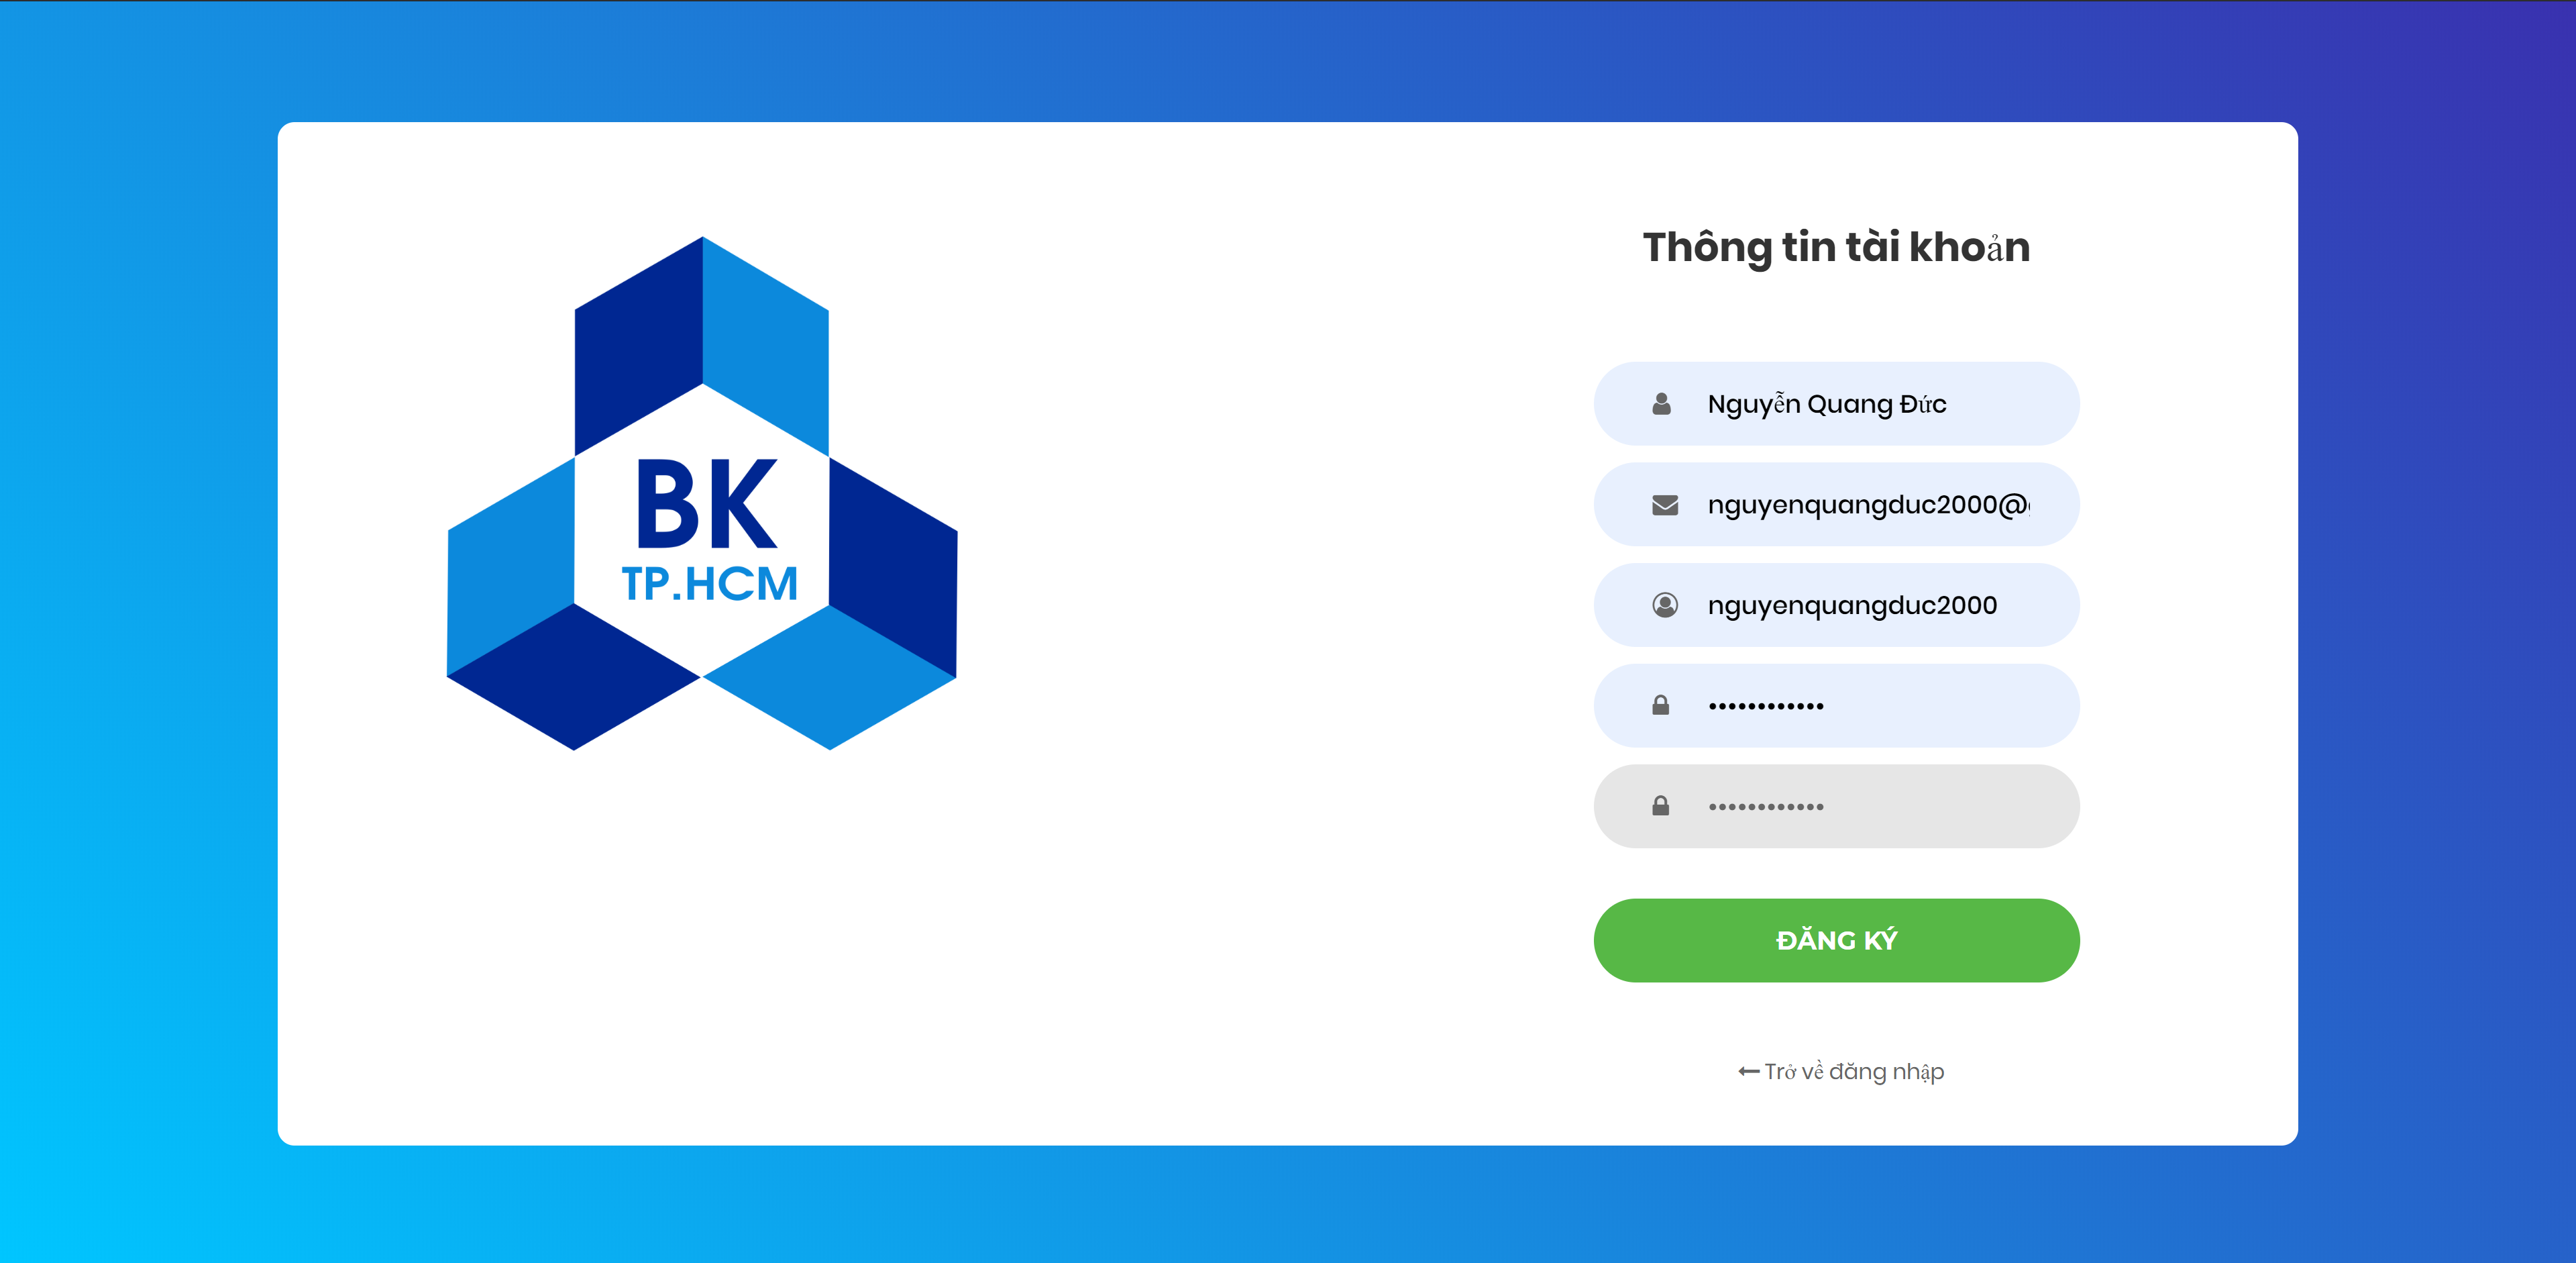
\includegraphics[scale=0.36]{create_user.png}
		\caption{Giao diện đăng ký tài khoản}
		\label{F:create_user}
	\end{figure}
	
	\begin{figure}[H]
		\centering
		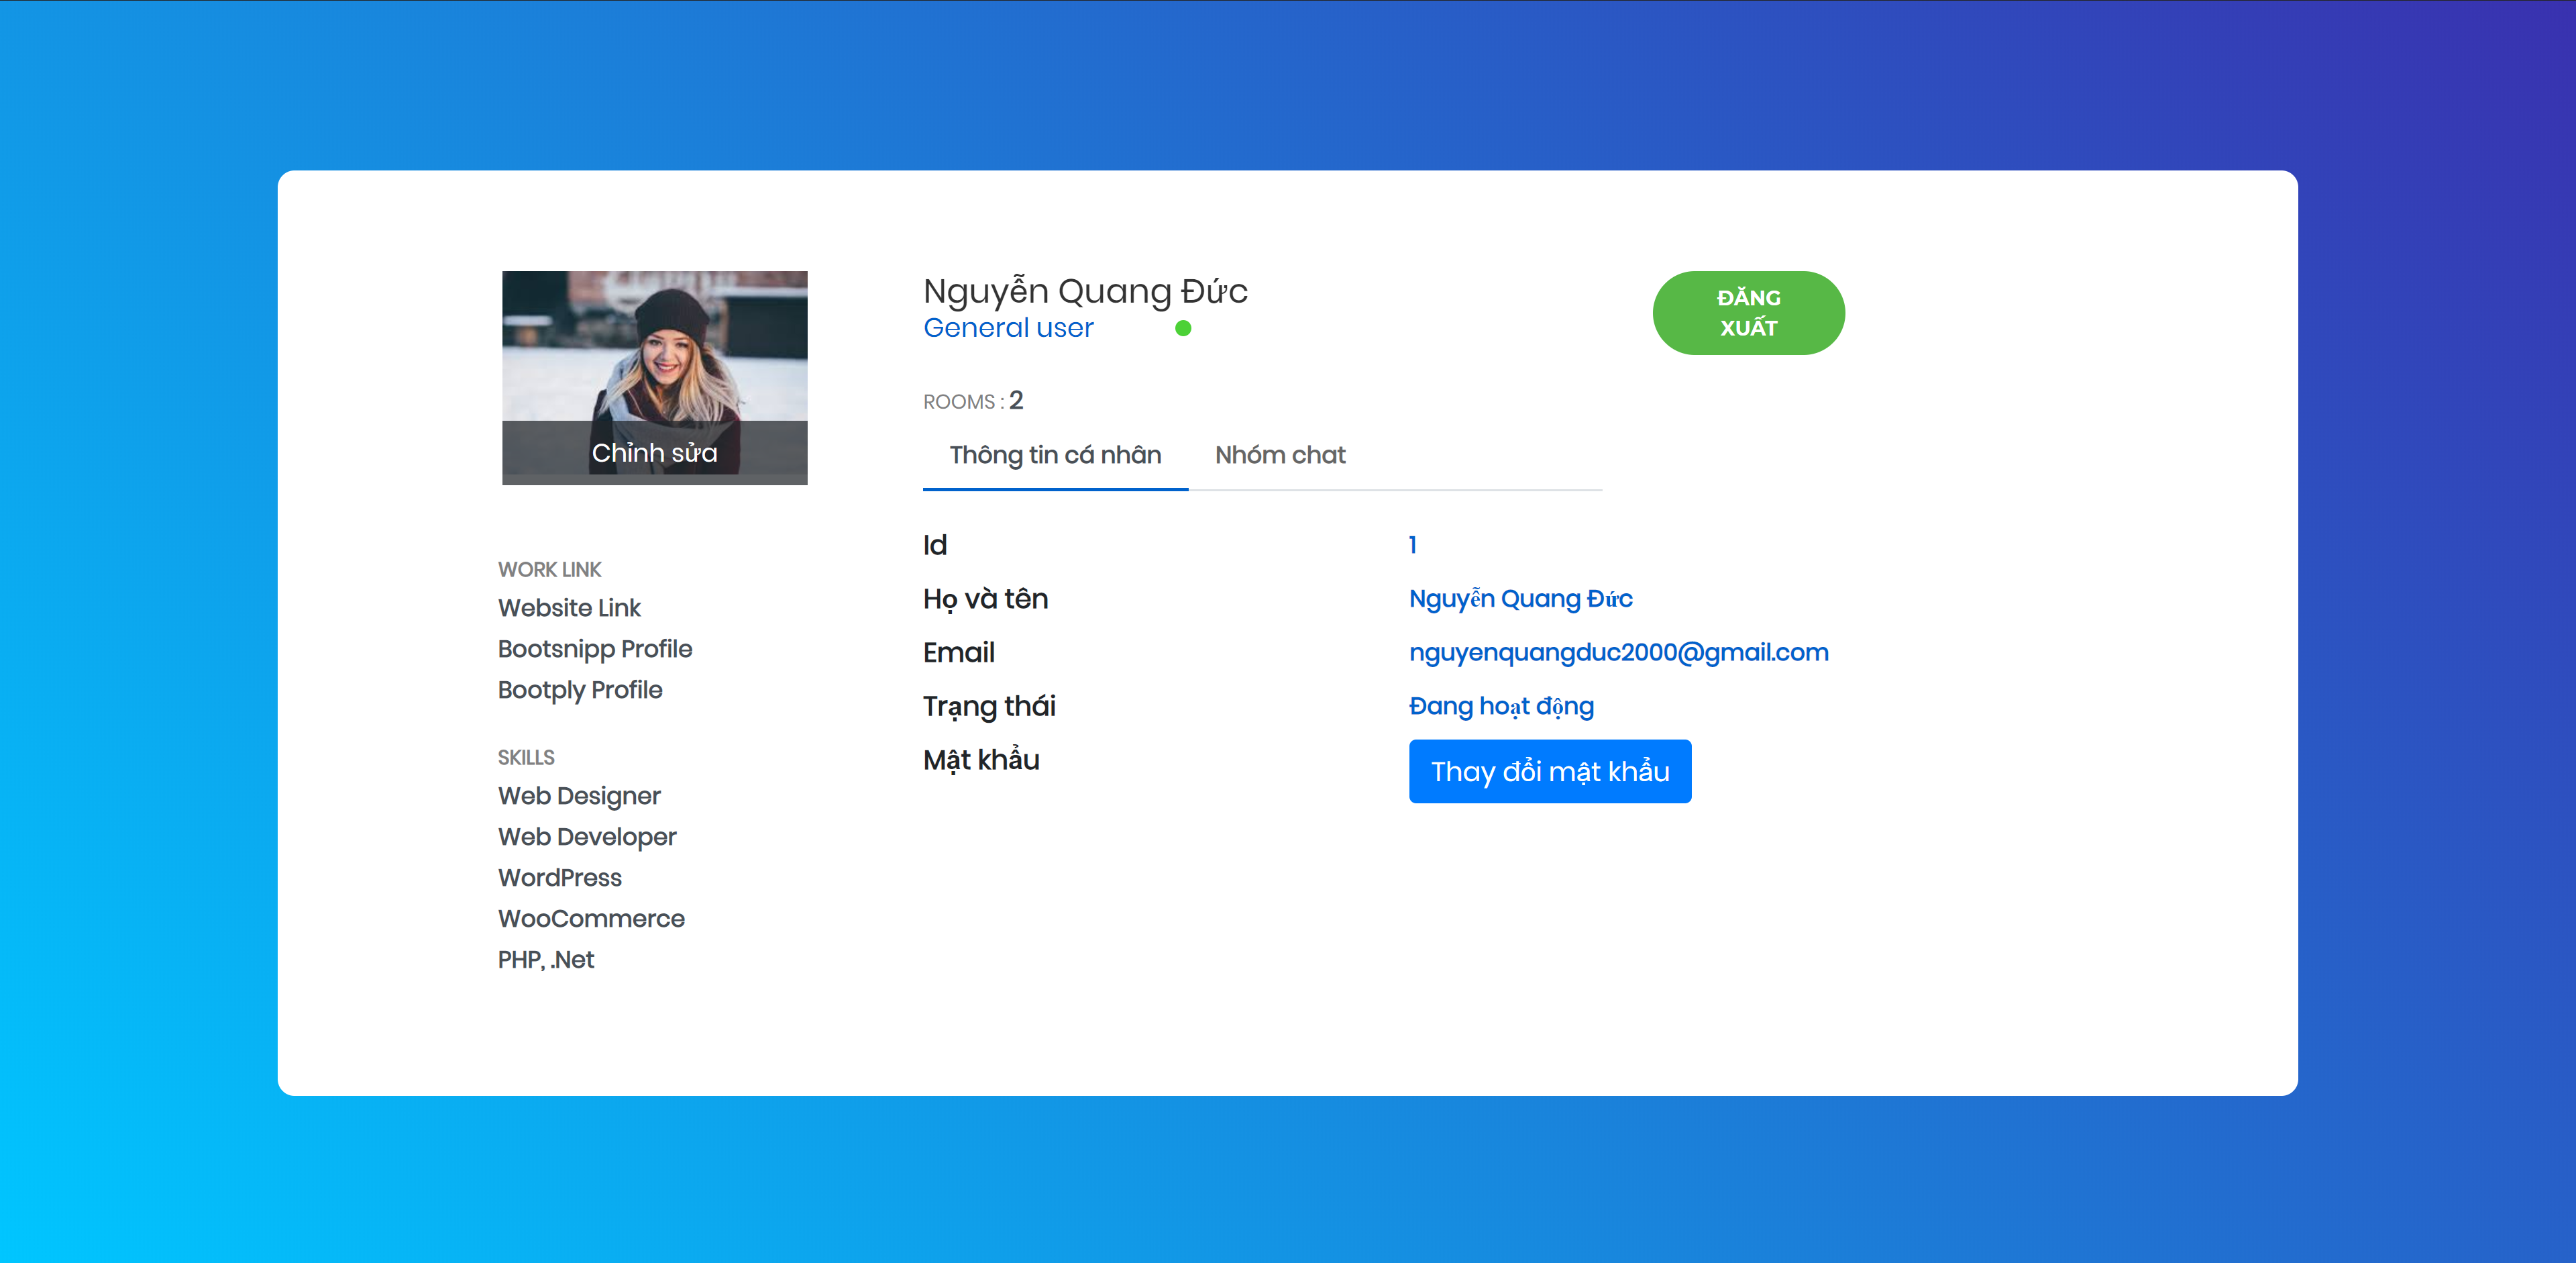
\includegraphics[scale=0.36]{profile_manager.png}
		\caption{Giao diện trang cá nhân khi đăng ký thành công}
		\label{F:profile_manager_register}
	\end{figure}
	
	\begin{figure}[H]
		\centering
		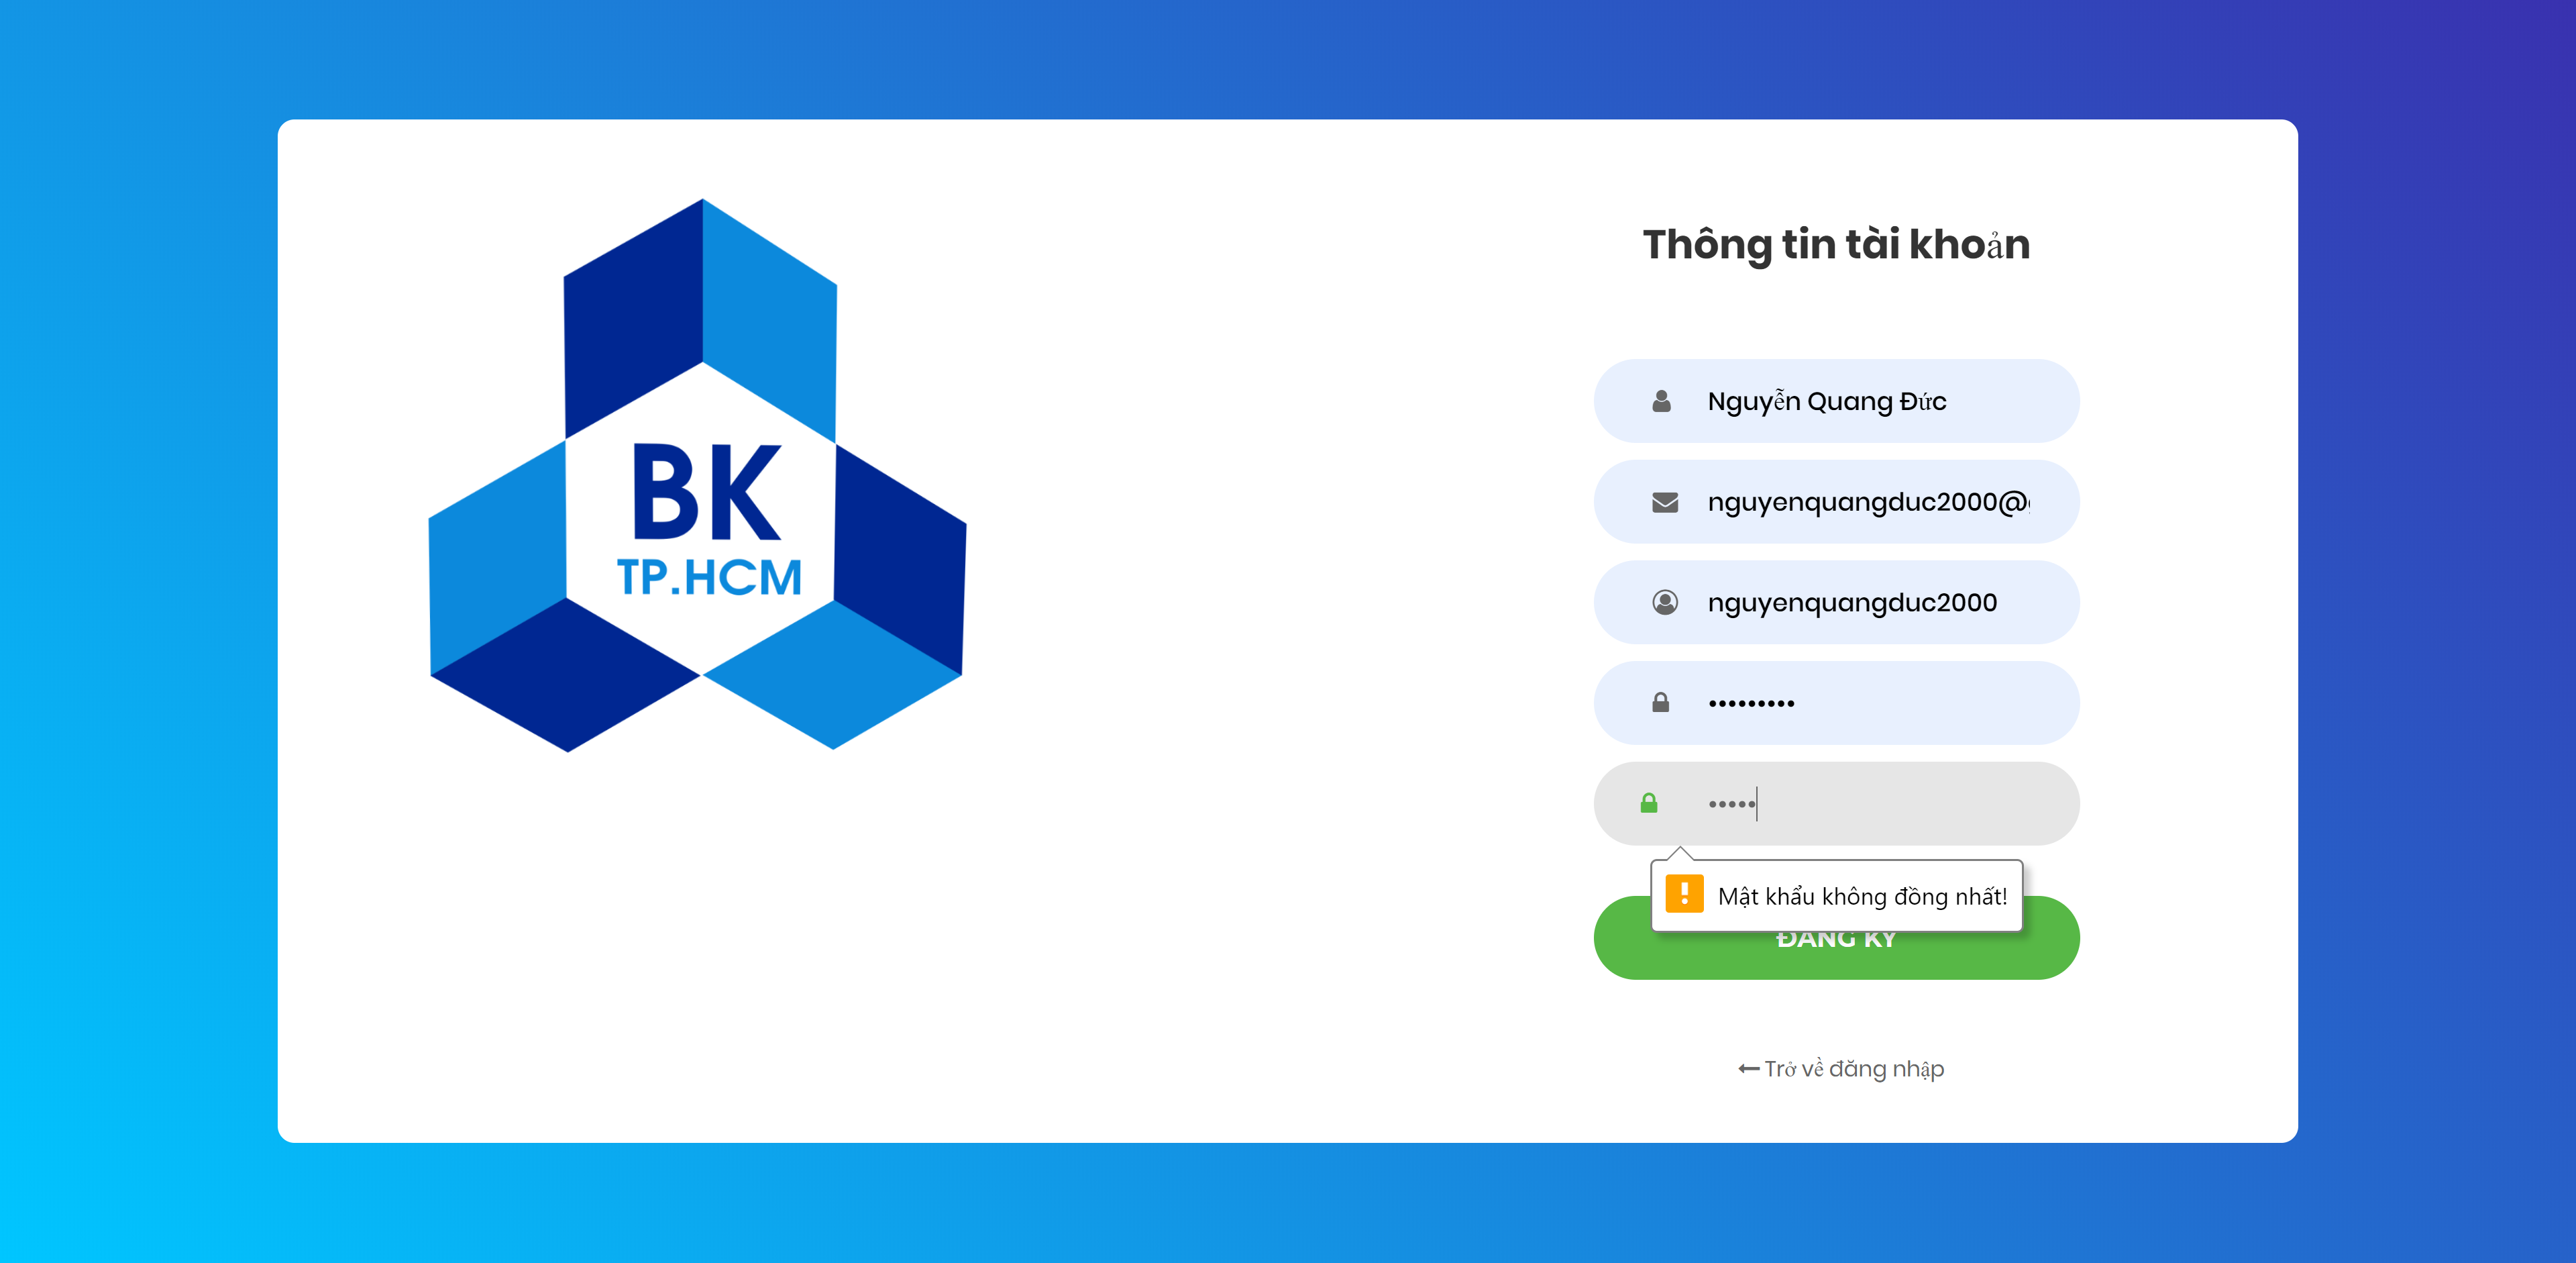
\includegraphics[scale=0.36]{password_not_match_register.png}
		\caption{Nếu nhập xác thực không trùng khớp}
		\label{F:password_not_match_register}
	\end{figure}
	
	\begin{figure}[H]
		\centering
		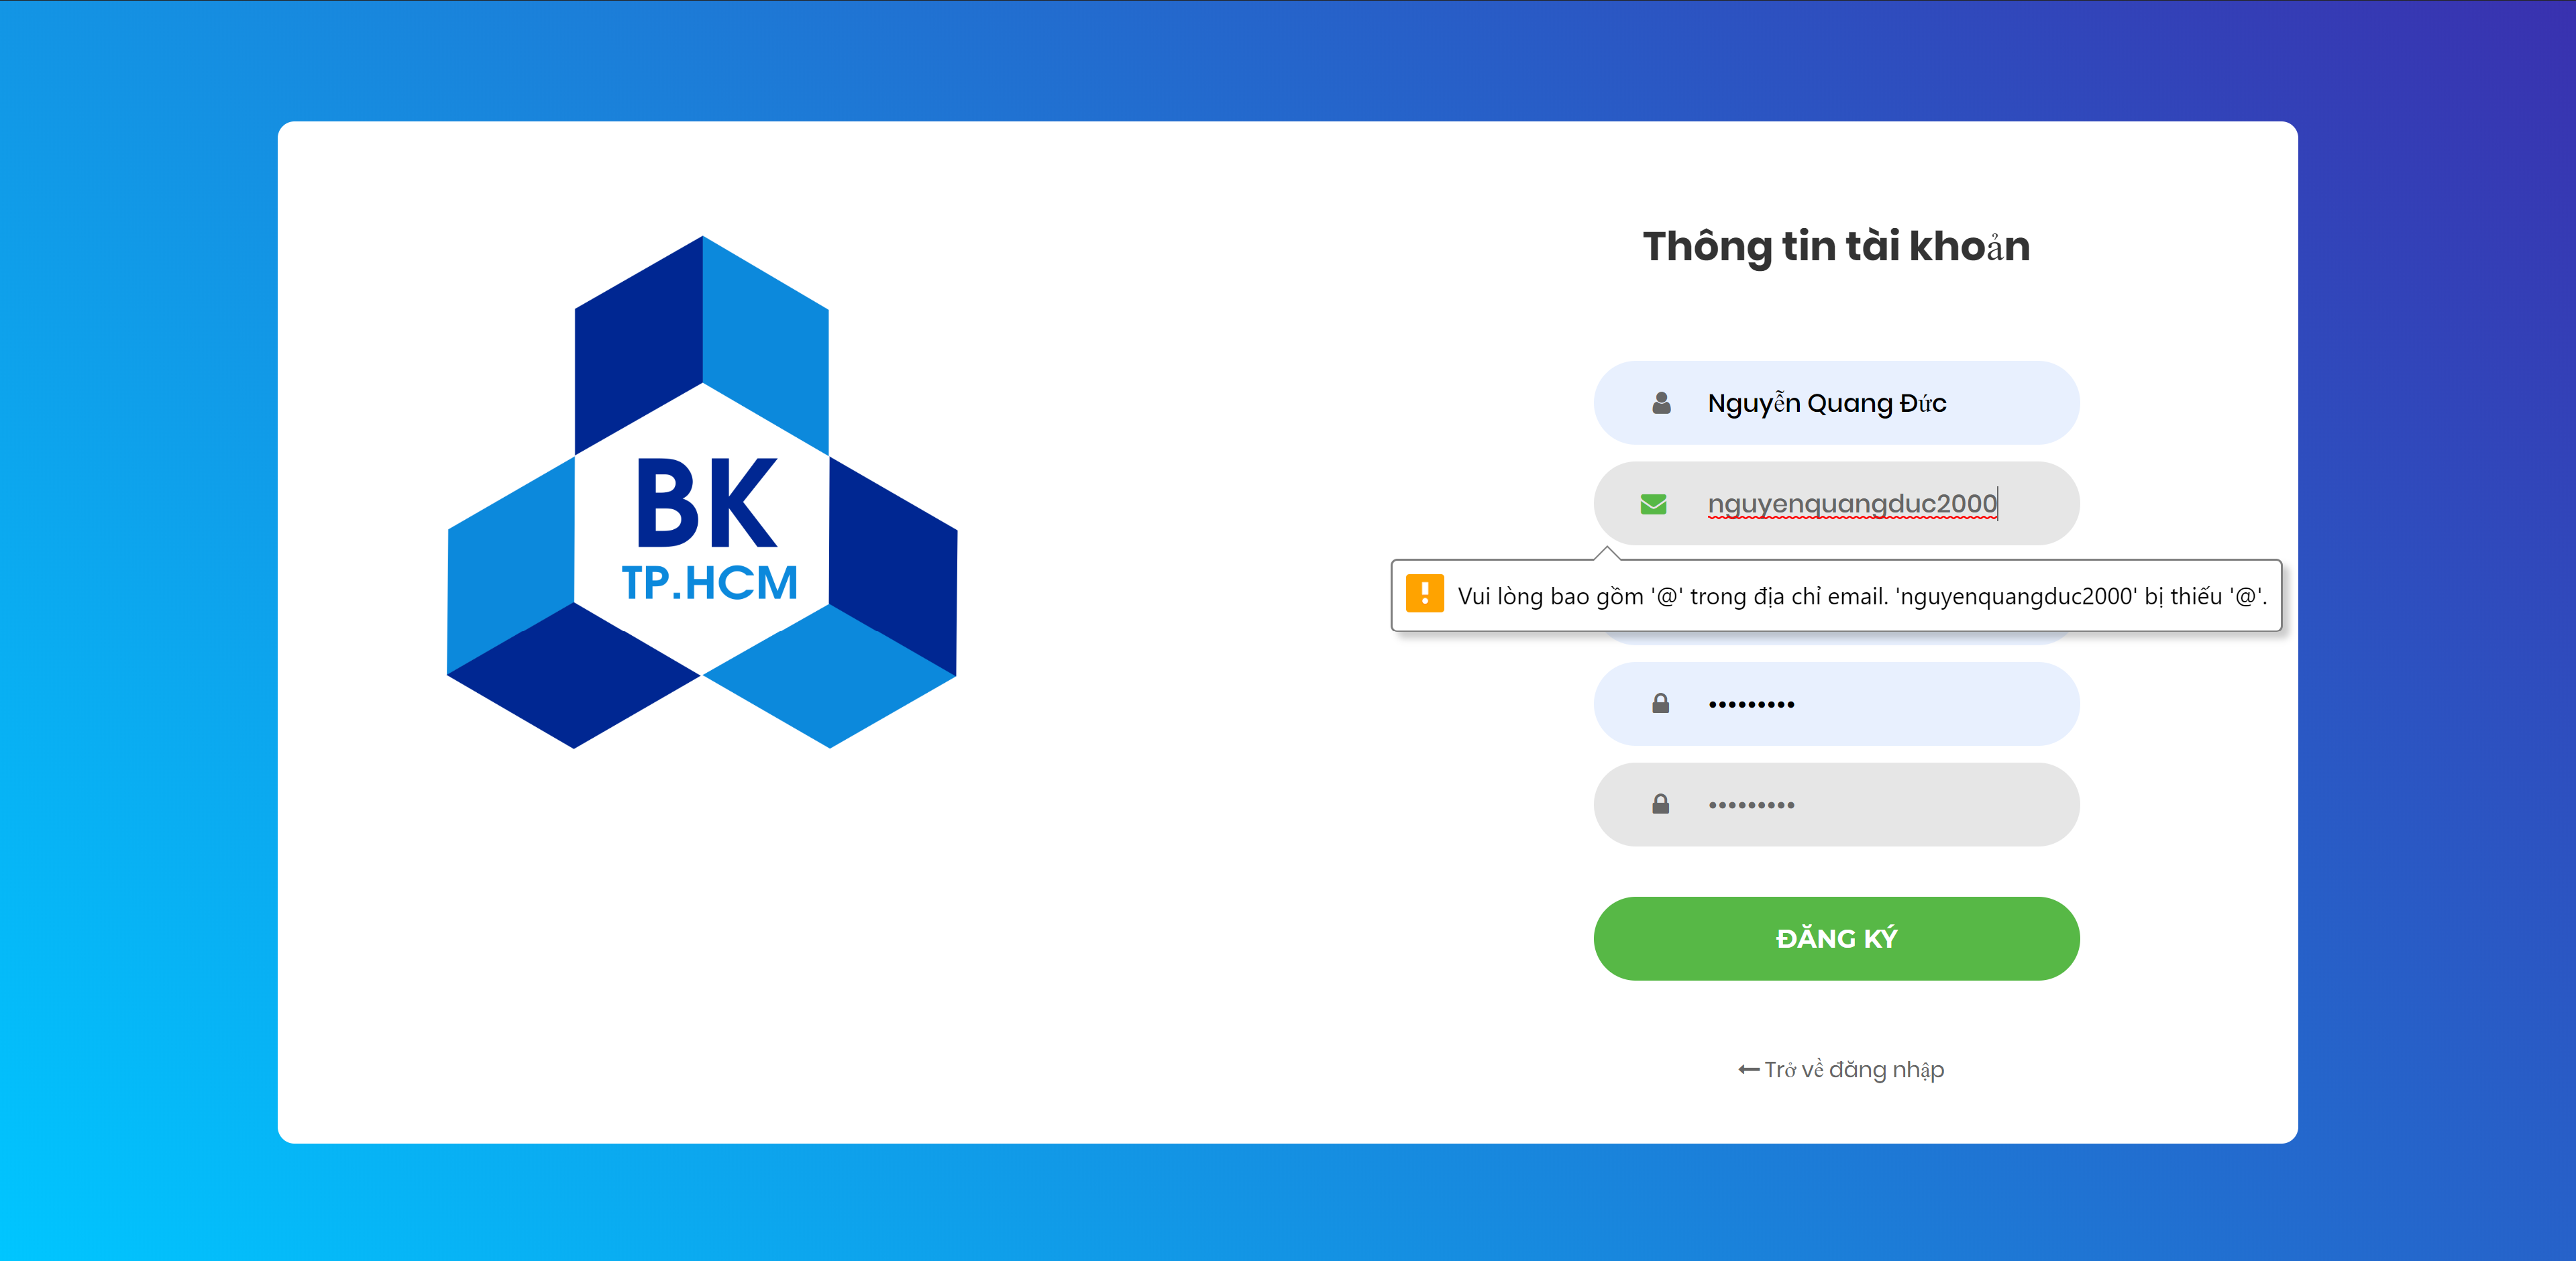
\includegraphics[scale=0.36]{check_email.png}
		\caption{Nếu nhập sai định dạng email}
		\label{F:check_email}
	\end{figure}
	
	\begin{figure}[H]
		\centering
		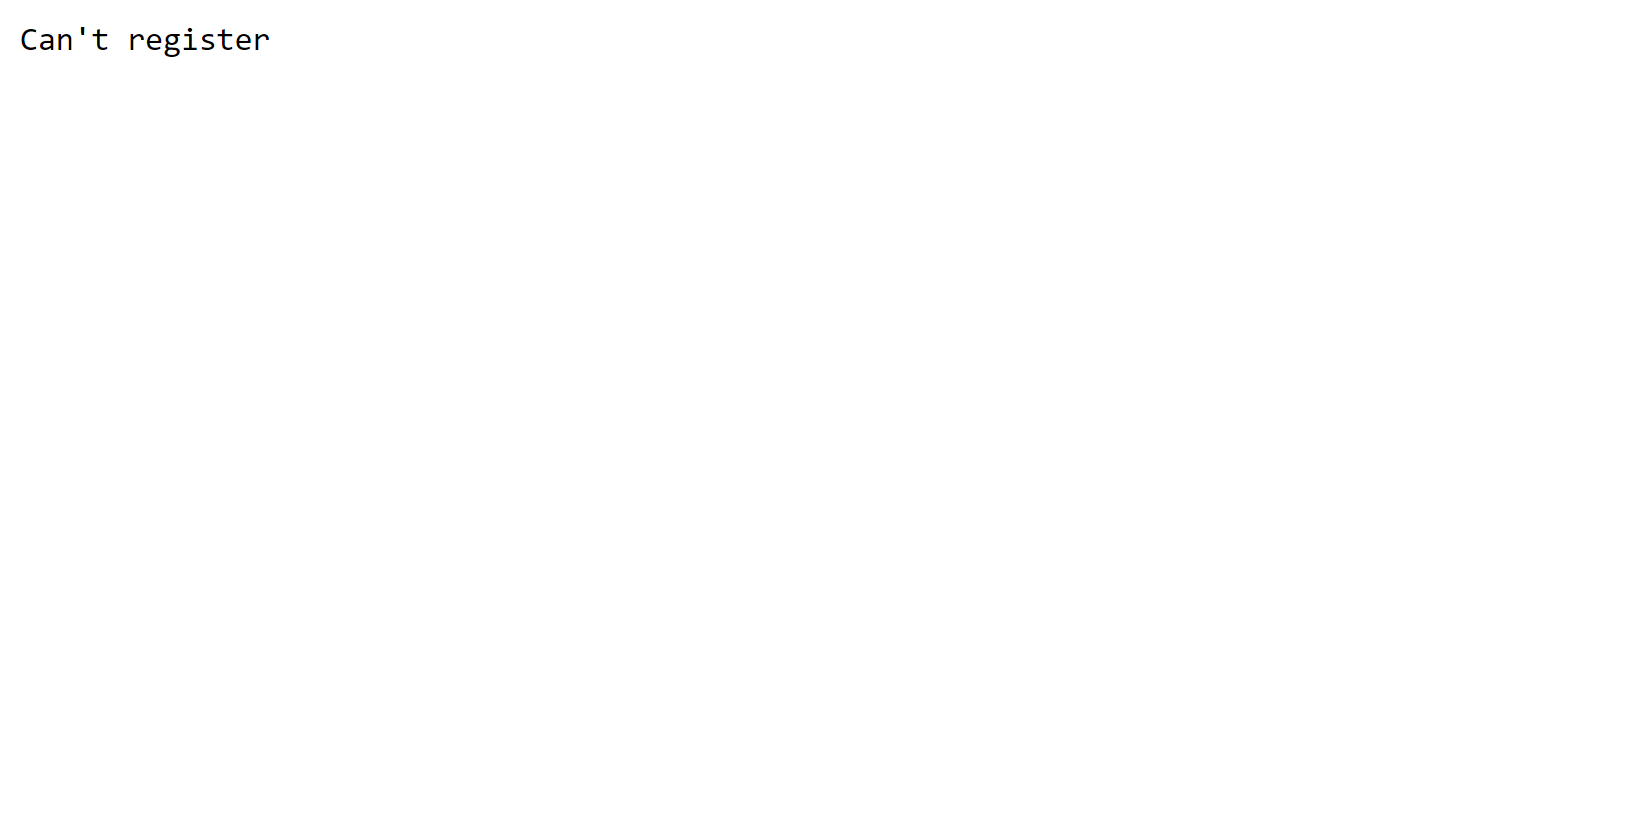
\includegraphics[scale=0.8]{can_not_register.png}
		\caption{Nếu tên người dùng hoặc email đã được đăng ký trước đó}
		\label{F:can_not_register}
	\end{figure}
	
	\subsection{Đăng nhập | Đăng xuất}
	Để đăng nhập, người dùng nhập vào tên người dùng và mật khẩu đã đăng ký trước đó. Nếu đăng nhập thành công, người dùng sẽ được chuyển đến trang cá nhân ngay sau đó.\linebreak
	Để đăng xuất, người dùng bấm vào nút "Đăng xuất" trên trang cá nhân. Sau khi đăng xuất, người dùng sẽ được chuyển hướng về trang đăng nhập.
	
	\begin{figure}[H]
		\centering
		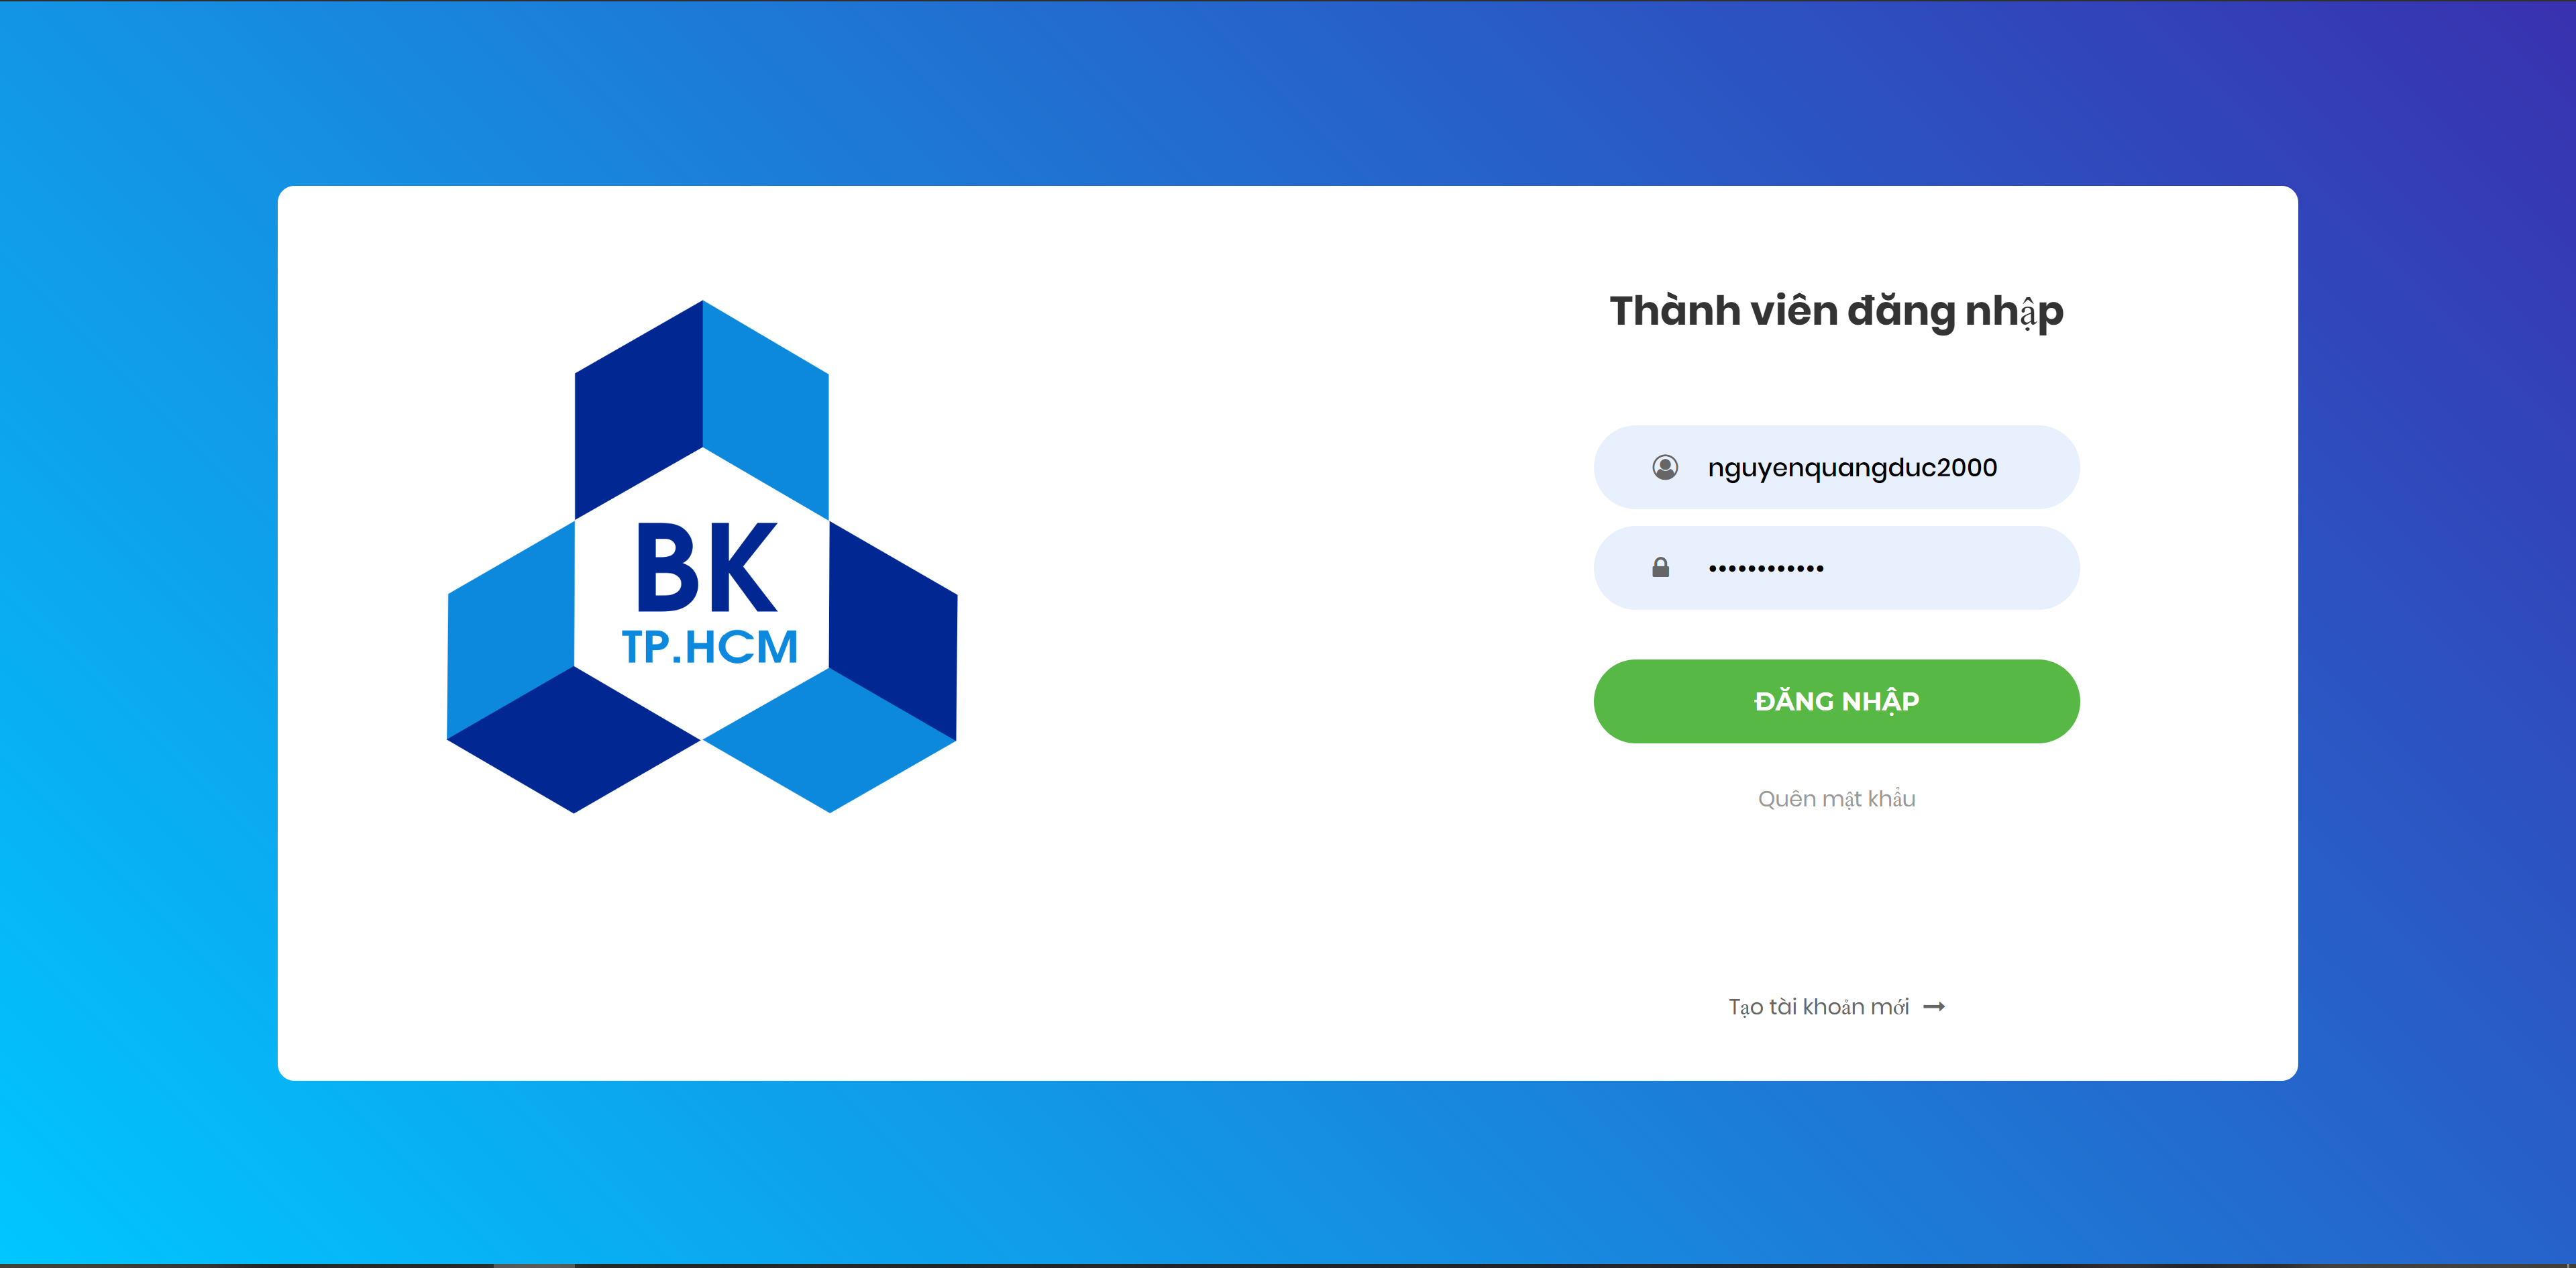
\includegraphics[scale=0.36]{login.png}
		\caption{Giao diện đăng nhập}
		\label{F:login}
	\end{figure}
	
	\begin{figure}[H]
		\centering
		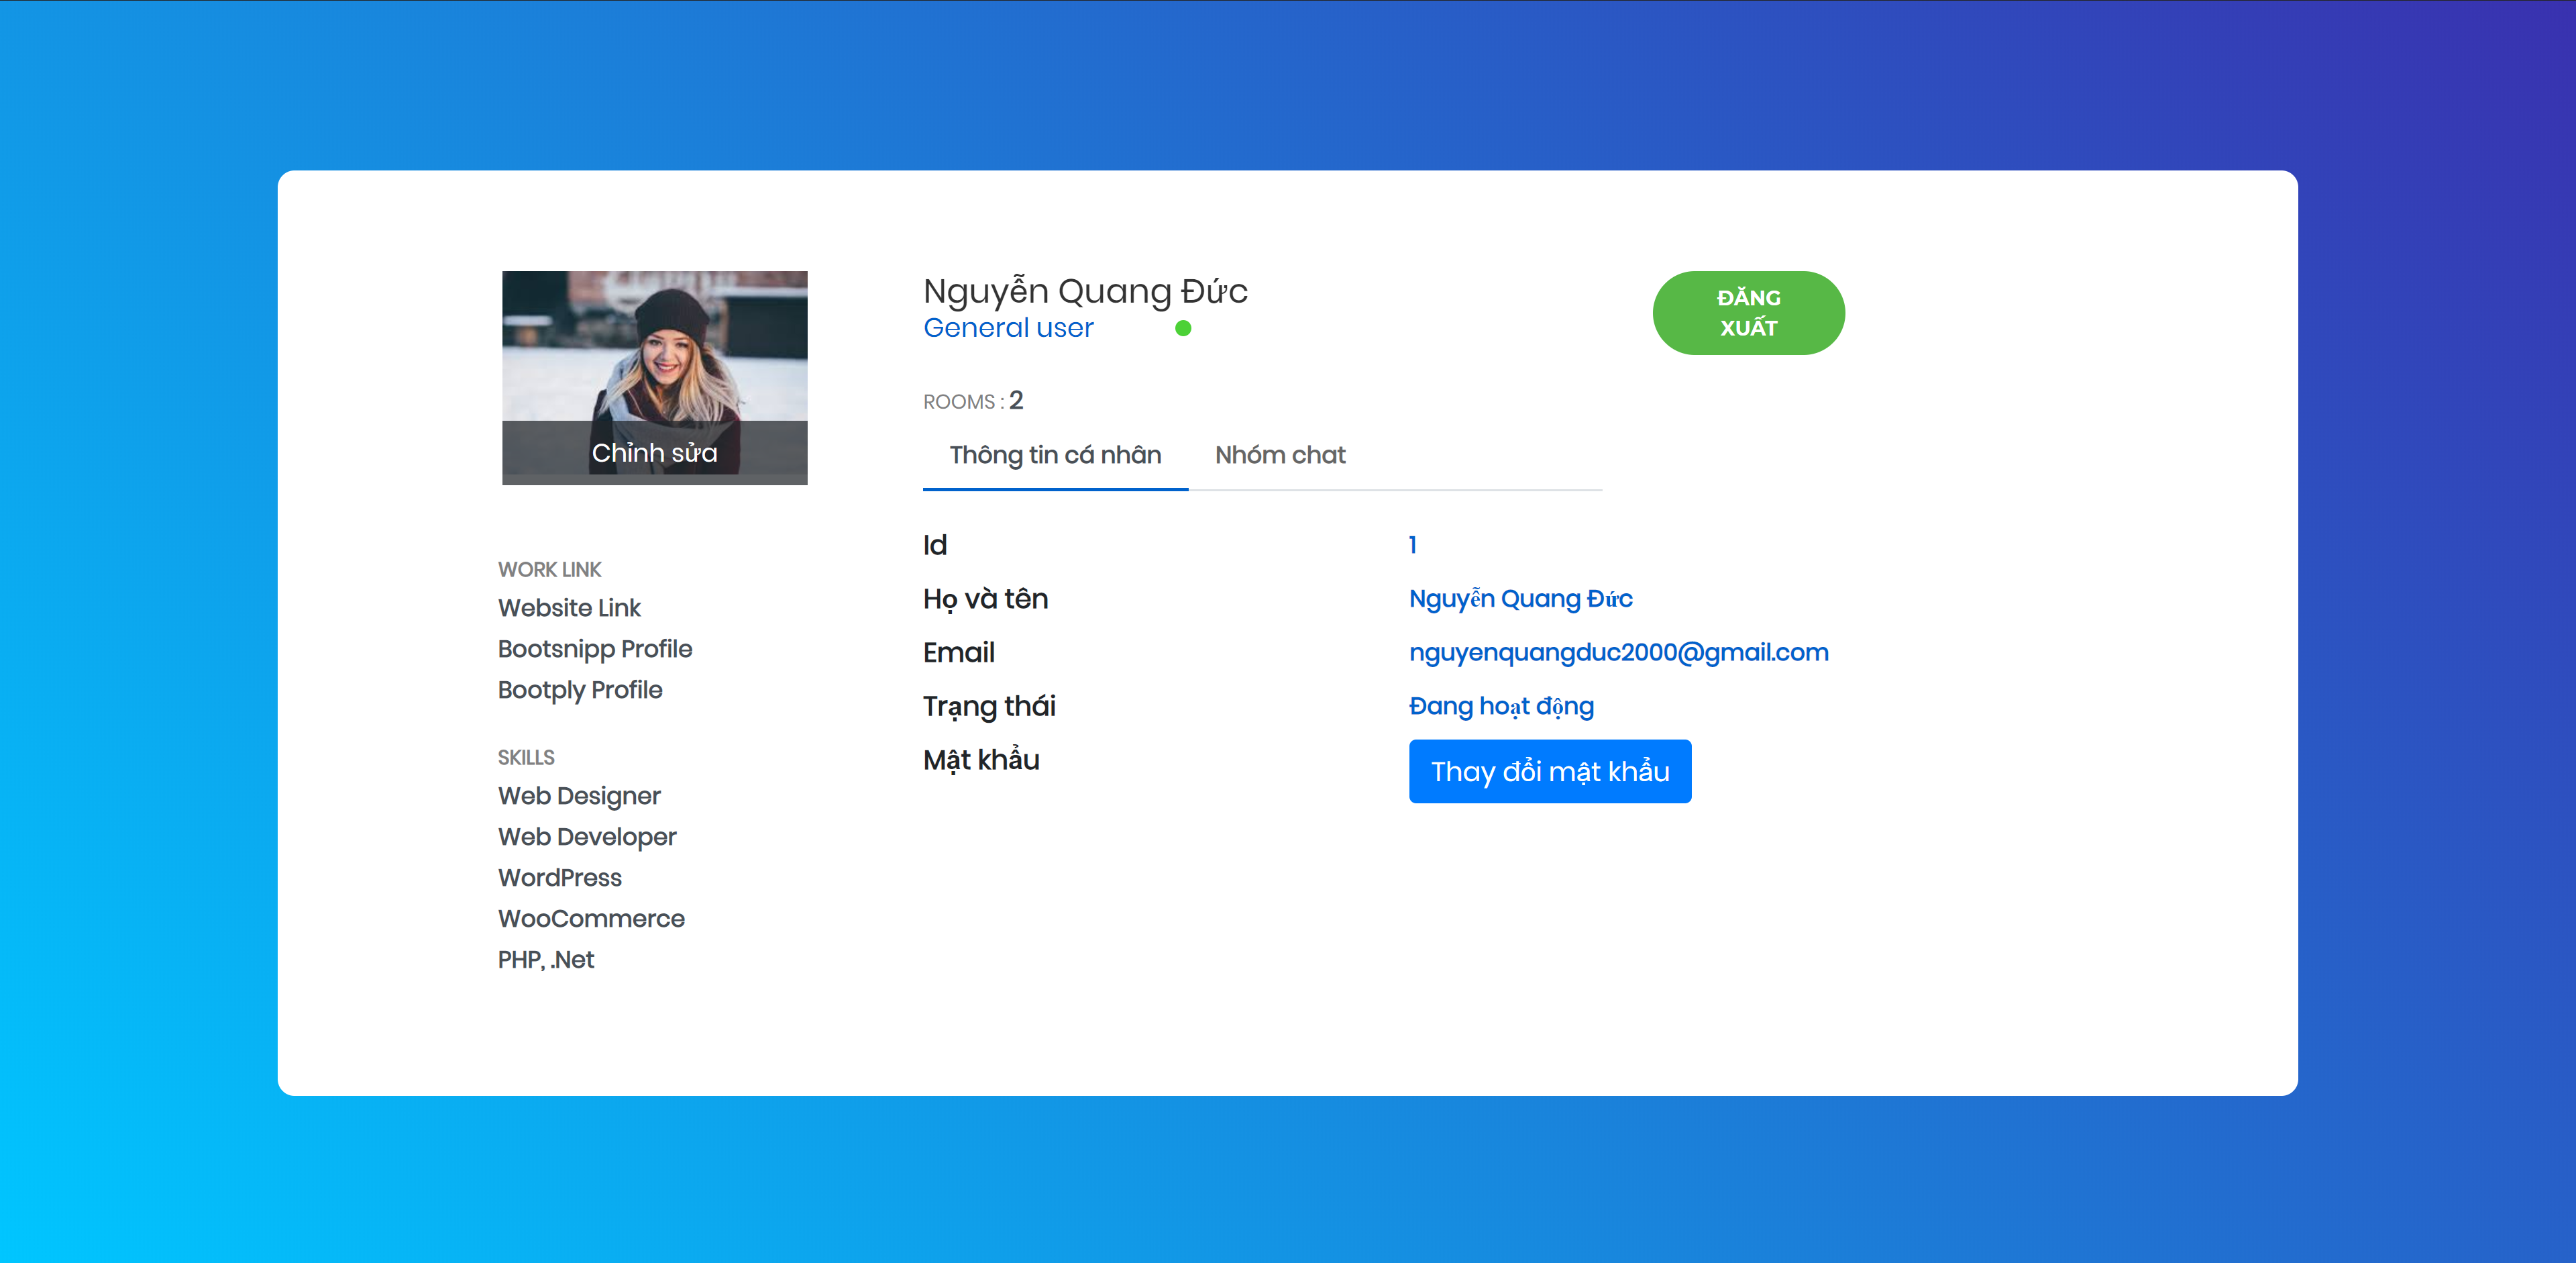
\includegraphics[scale=0.36]{profile_manager.png}
		\caption{Giao diện trang cá nhân khi đăng nhập thành công}
		\label{F:profile_manager_login}
	\end{figure}
	
	\begin{figure}[H]
		\centering
		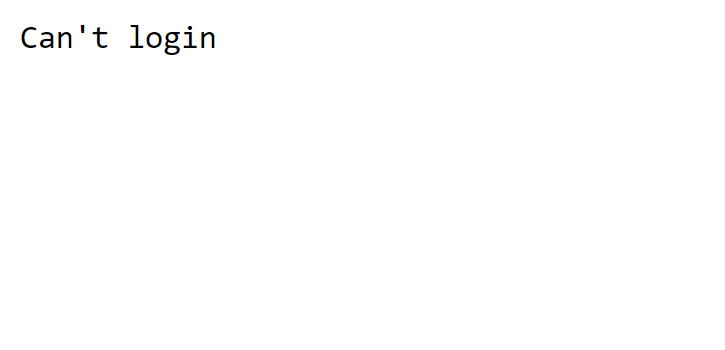
\includegraphics[scale=1]{can_not_login.png}
		\caption{Nếu tên người dùng hoặc mật khẩu đã nhập sai hoặc không có}
		\label{F:can_not_login}
	\end{figure}
	
	\subsection{Quên mật khẩu}
	Nếu người dùng quên mật khẩu có thể lấy lại mật khẩu bằng cách chọn "Quên mật khẩu" tại trang đăng nhập. Sau đó nhập địa chỉ email đã đăng ký trước đó vào.\linebreak
	
	\begin{figure}[H]
		\centering
		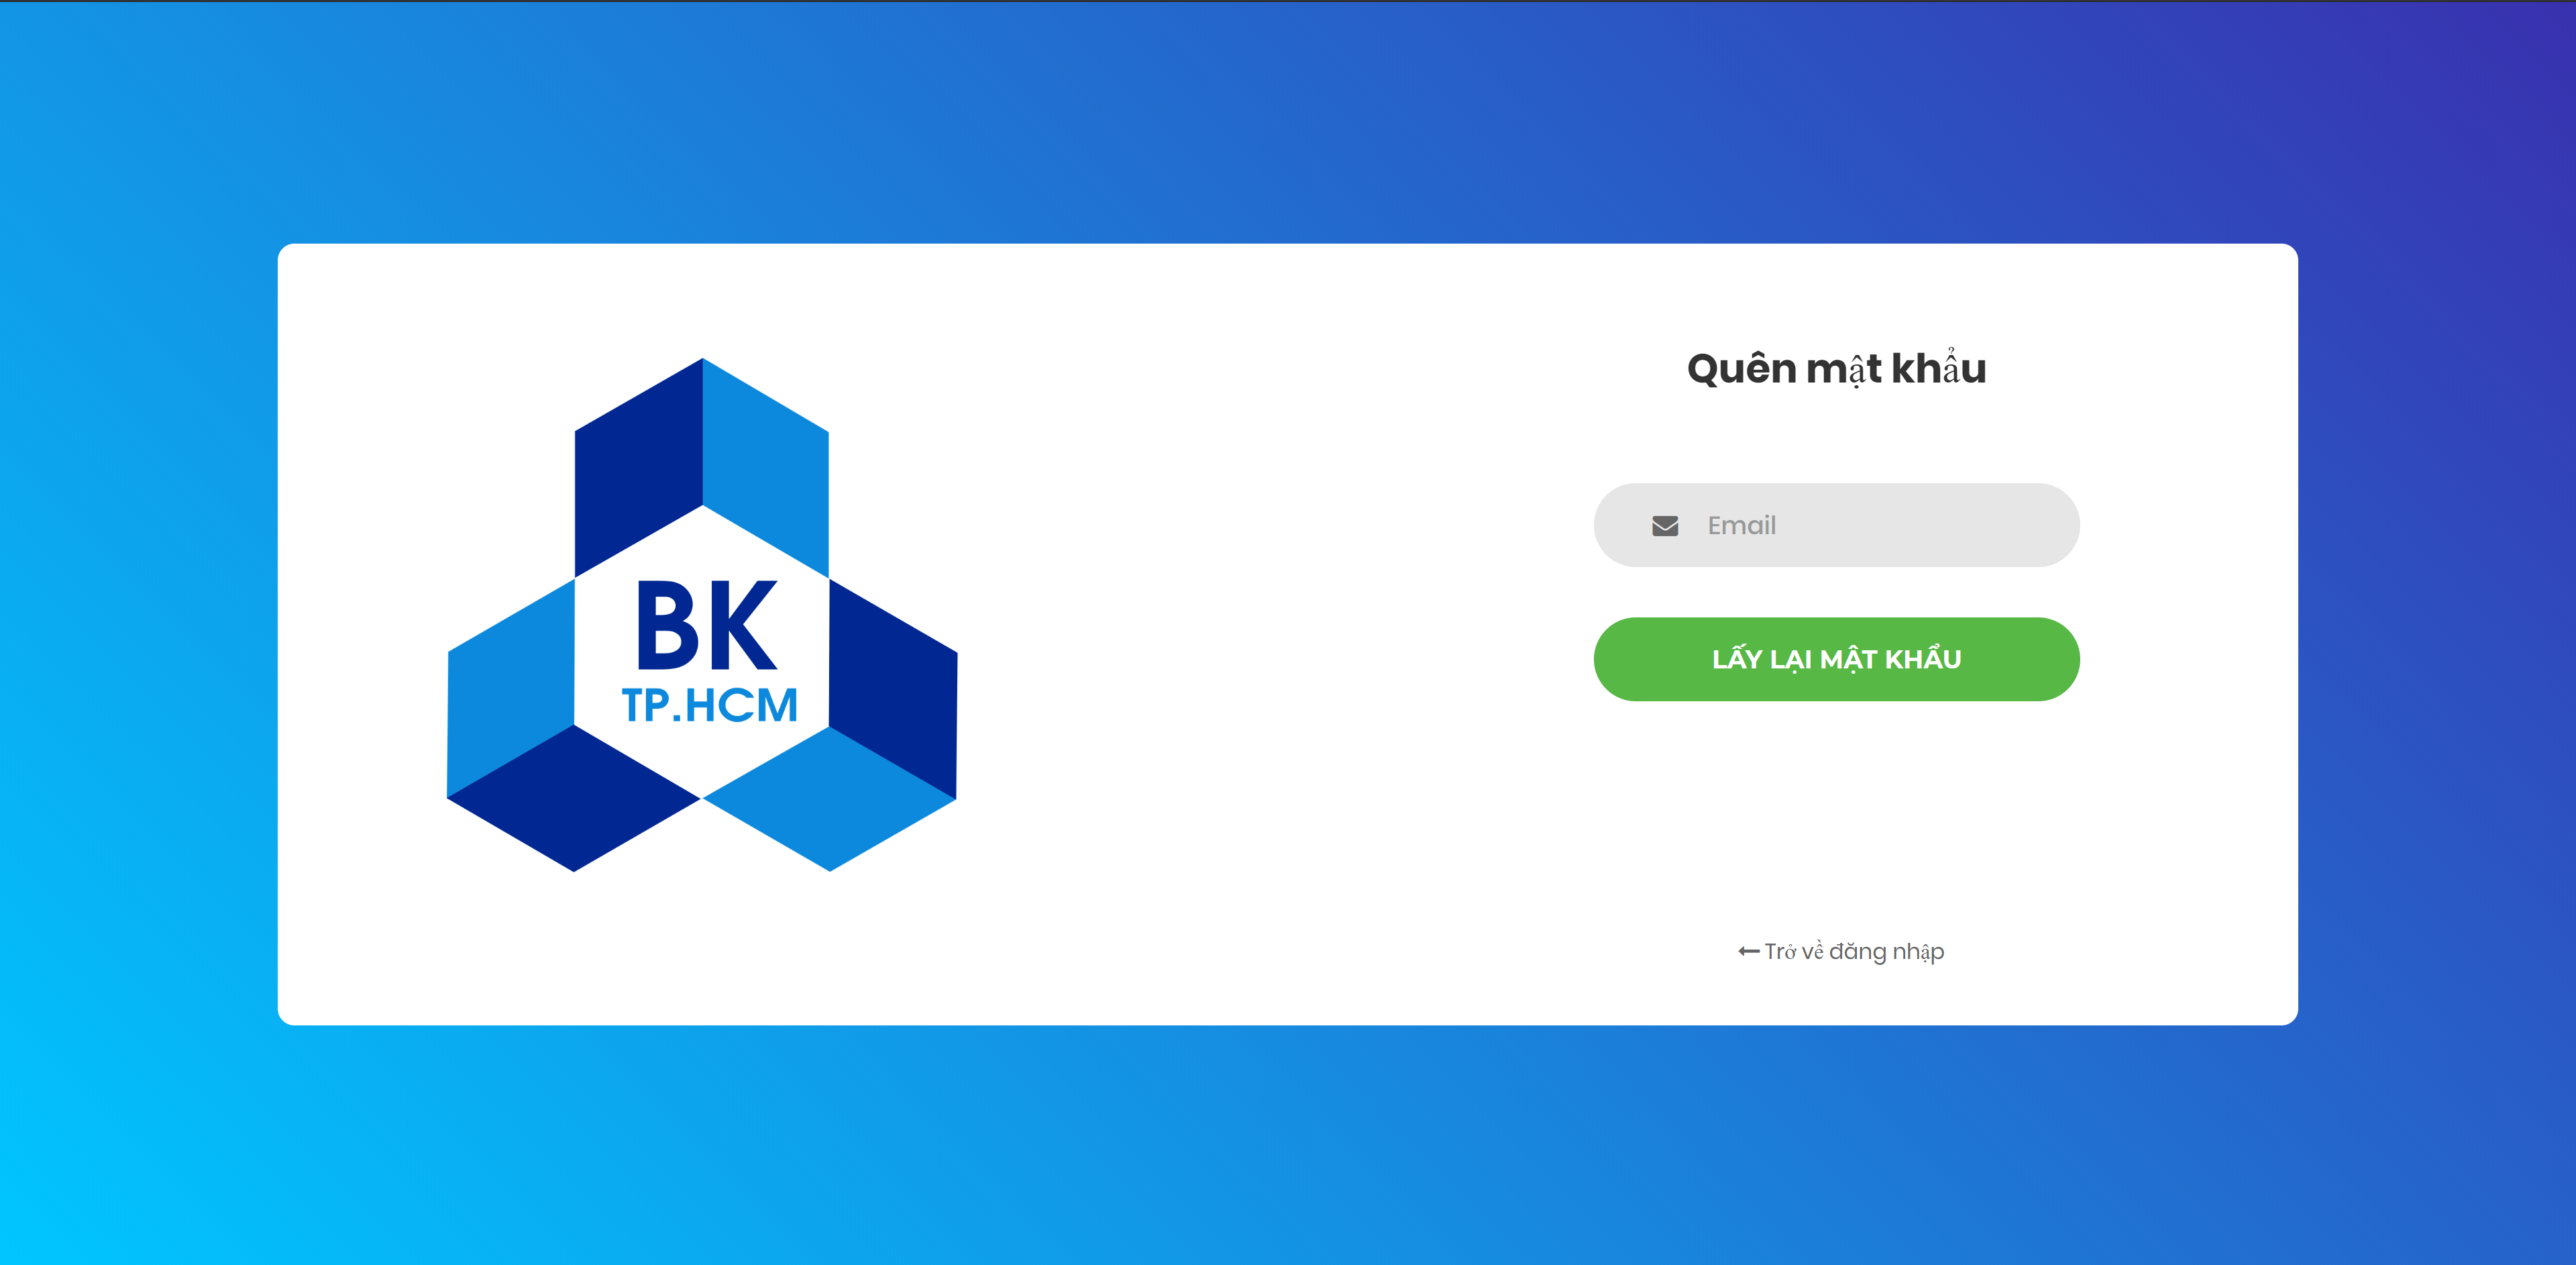
\includegraphics[scale=0.36]{forget_password.png}
		\caption{Nhập email vào để lấy lại mật khẩu}
		\label{F:forget_password}
	\end{figure}
	
	\begin{figure}[H]
		\centering
		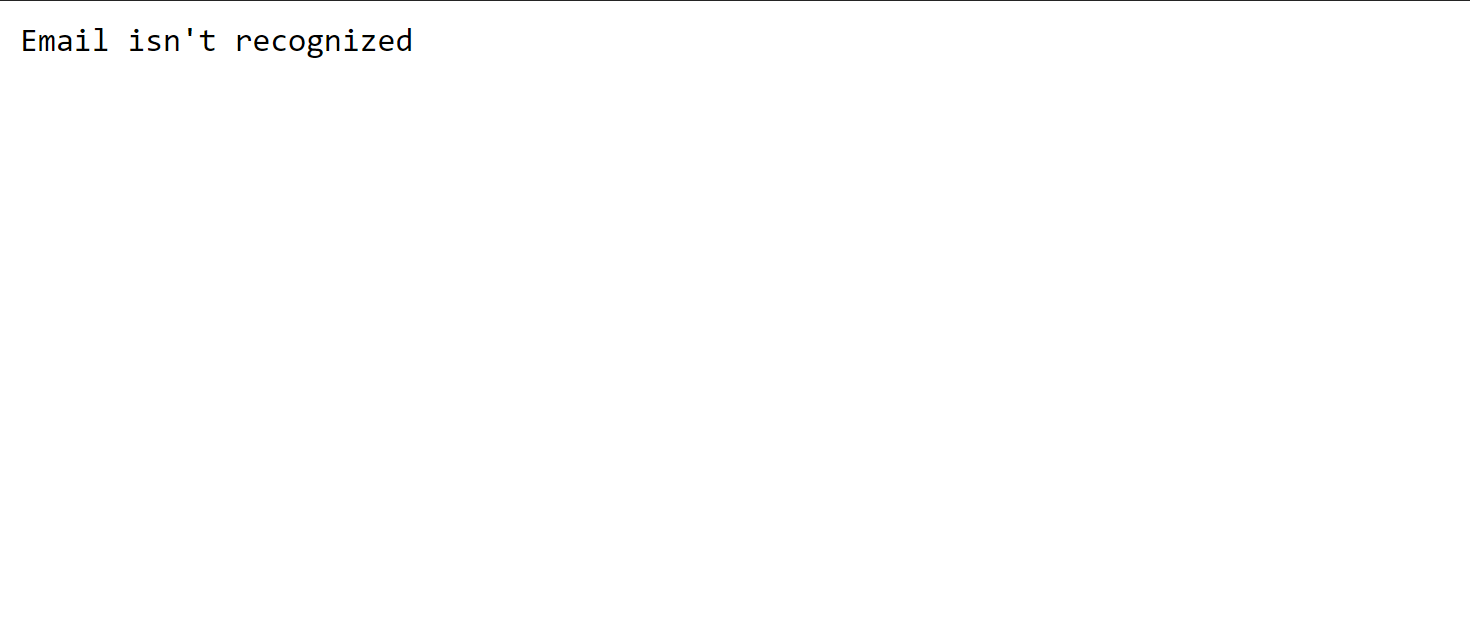
\includegraphics[scale=0.8]{email_not_reconize.png}
		\caption{Trong trường hợp nhập sai email hoặc email chưa được đăng ký}
		\label{F:email_not_reconize}
	\end{figure}
	
	\subsection{Thay đổi mật khẩu}
	Để thay đổi mật khẩu, người dùng đăng nhập vào trang cá nhân. Tại mục "Mật khẩu" chọn "Thay đổi mật khẩu".\linebreak
	Người dùng nhập mật khẩu cũ và mật khẩu mới vào và bấm "Xác nhận". Nếu mật khẩu cũ hợp lệ thì mật khẩu sẽ được thay đổi, sau khi thay đổi, người dùng vẫn ở trang cá nhân. Ngược lại, người dùng sẽ bị đăng xuất ra khỏi hệ thống nhằm đảm bảo tính bảo mật.
	
	\begin{figure}[H]
		\centering
		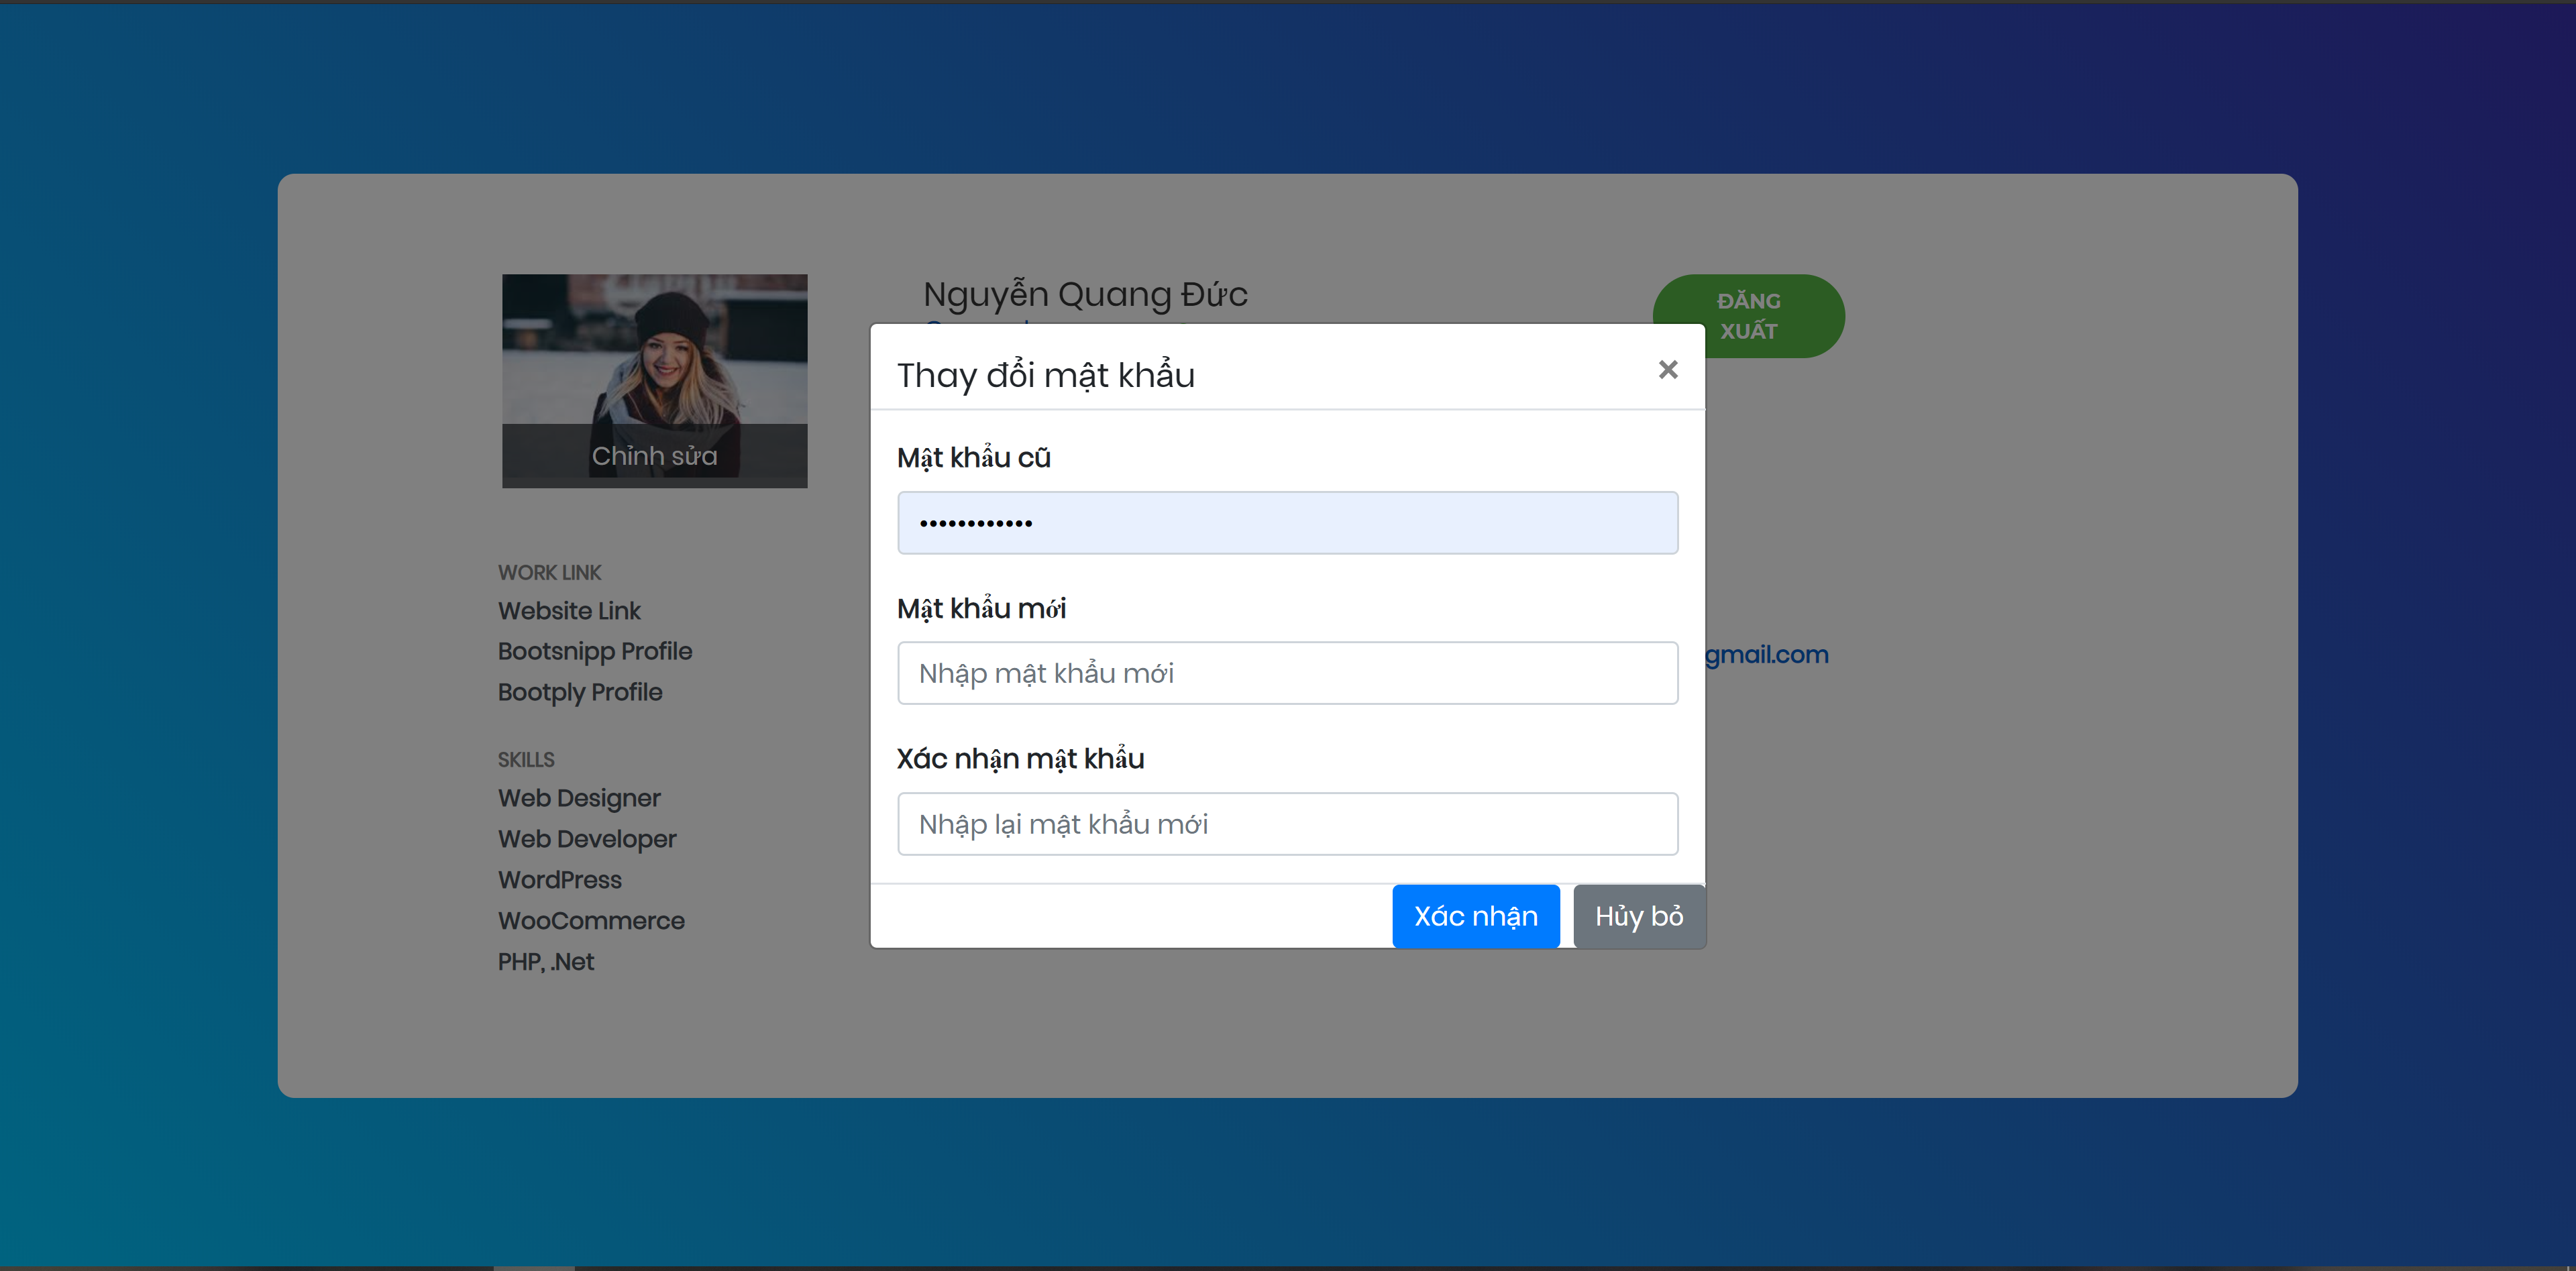
\includegraphics[scale=0.36]{change_password.png}
		\caption{Thay đổi mật khẩu}
		\label{F:change_password}
	\end{figure}
	
	\begin{figure}[H]
		\centering
		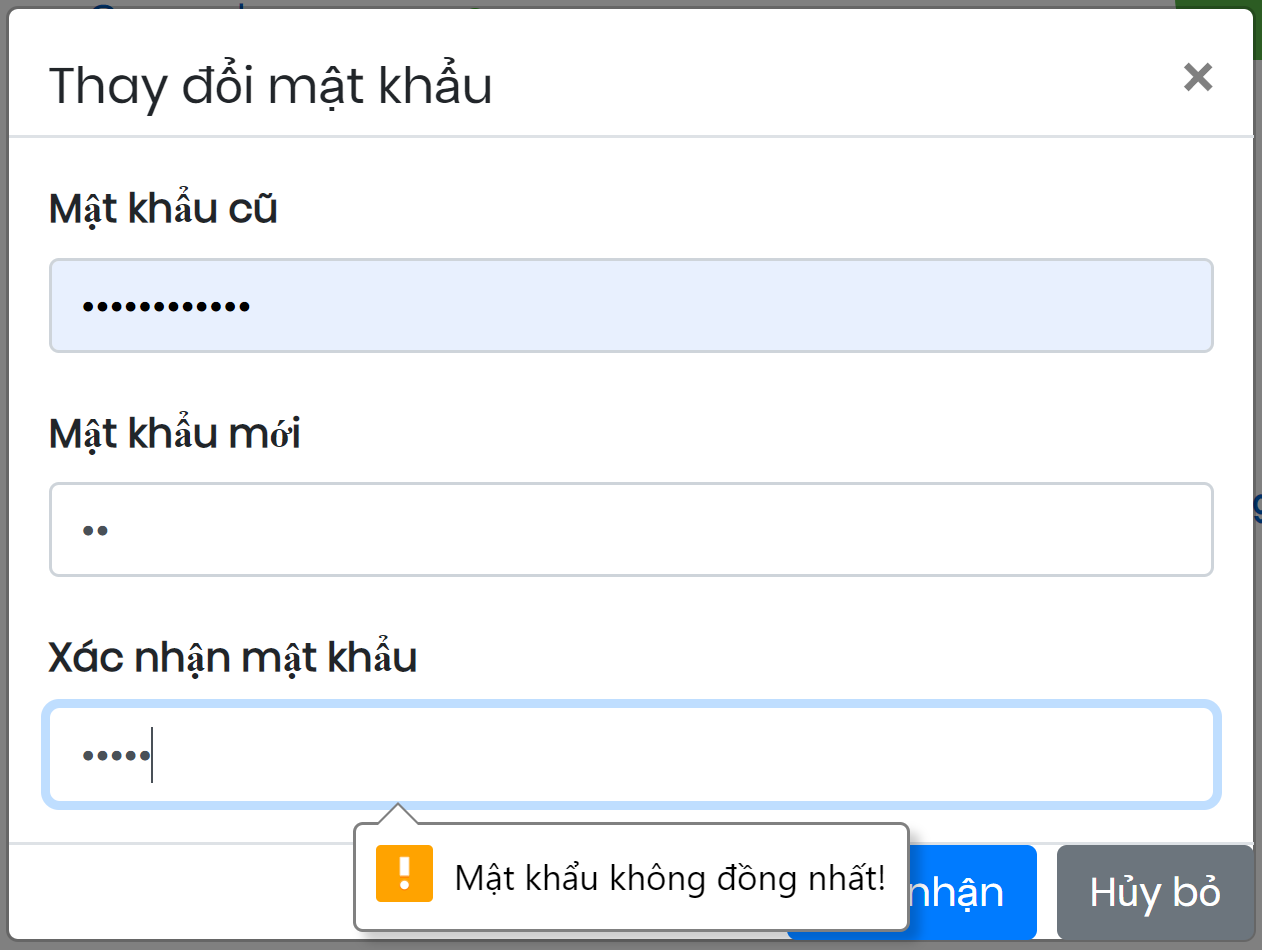
\includegraphics[scale=0.8]{password_not_match.png}
		\caption{Xác thực mật khẩu mới phải trùng với nhau}
		\label{F:password_not_match}
	\end{figure}
	
	\subsection{Tạo phòng chat}
	Để tạo phòng chat, tại trang cá nhân, người dùng chọn tab "Nhóm chat". Sau đó bấm nút "Tạo phòng chat".\linebreak
	Người dùng nhập tên phòng chat và bấm nút "Tạo phòng".
	
	\begin{figure}[H]
		\centering
		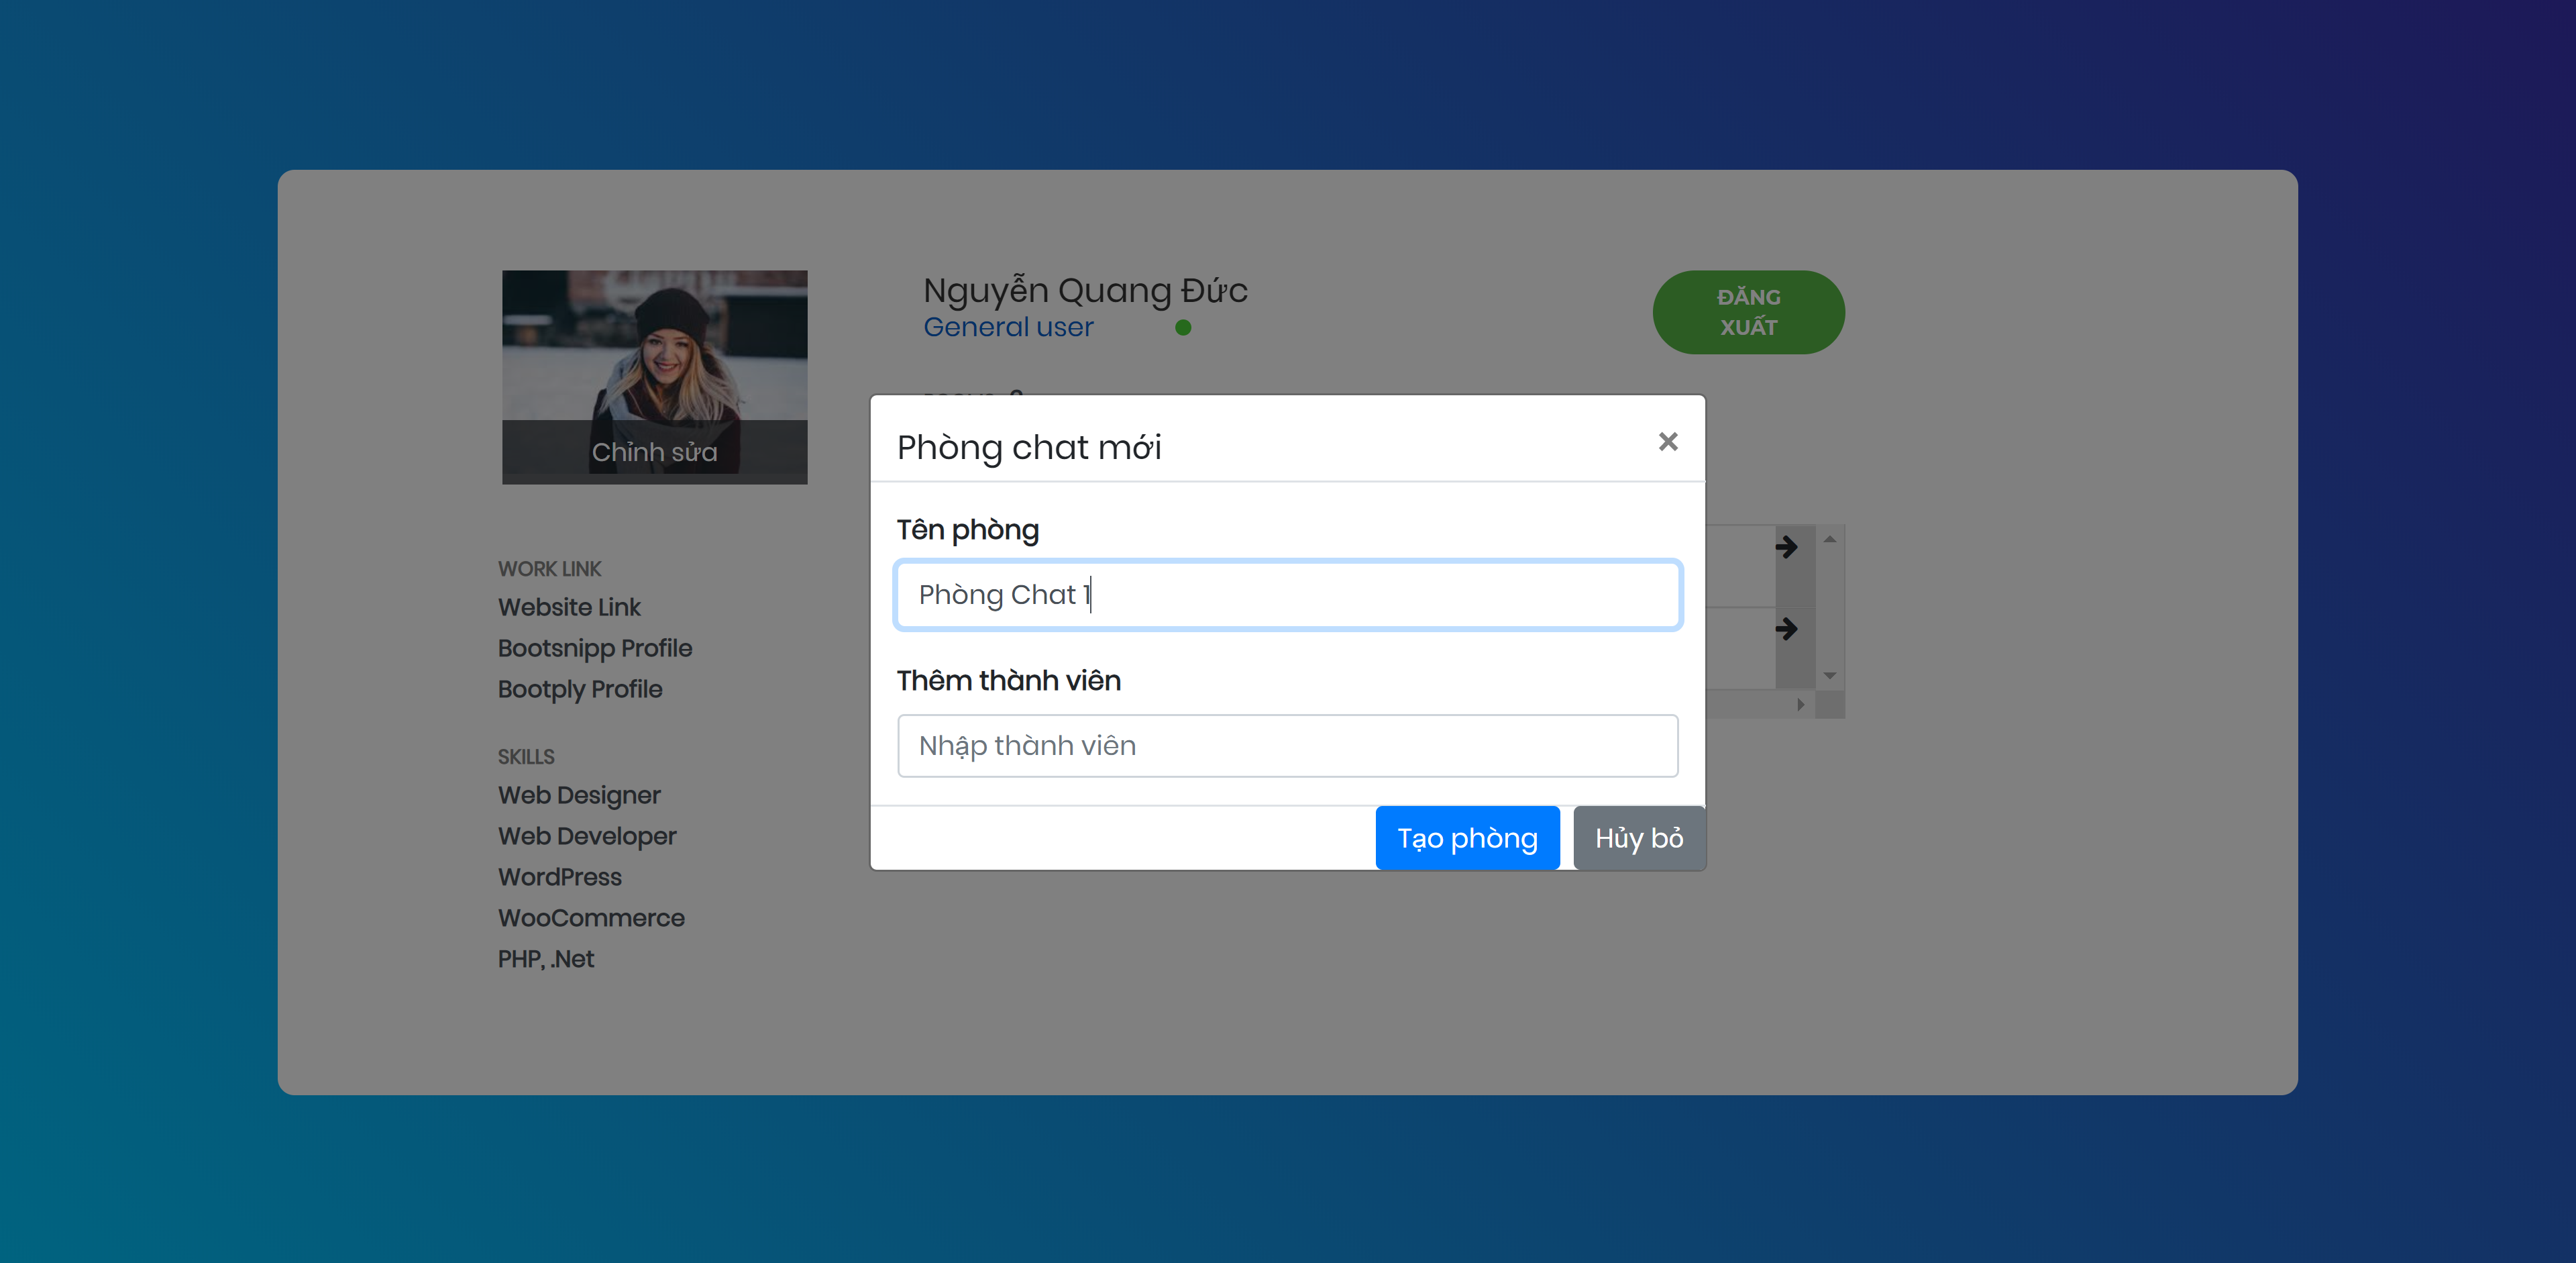
\includegraphics[scale=0.36]{create_room.png}
		\caption{Tạo phòng chat}
		\label{F:create_room}
	\end{figure}
	
	\subsection{Thêm bạn bè vào phòng chat}
	Để thêm bạn bè vào phòng chat, hãy nhập tên người dùng của họ vào mục "Thêm thành viên". Nếu có nhiều bạn bè, hãy nhập phân biệt bằng dấu ','.\linebreak
	Bạn bè chỉ có thể thêm vào phòng chat khi bạn nhập đúng tên người dùng của họ và chắc chắn rằng tên người dùng đó đã đăng ký tài khoản trên ứng dụng chat này.
	
	\begin{figure}[H]
		\centering
		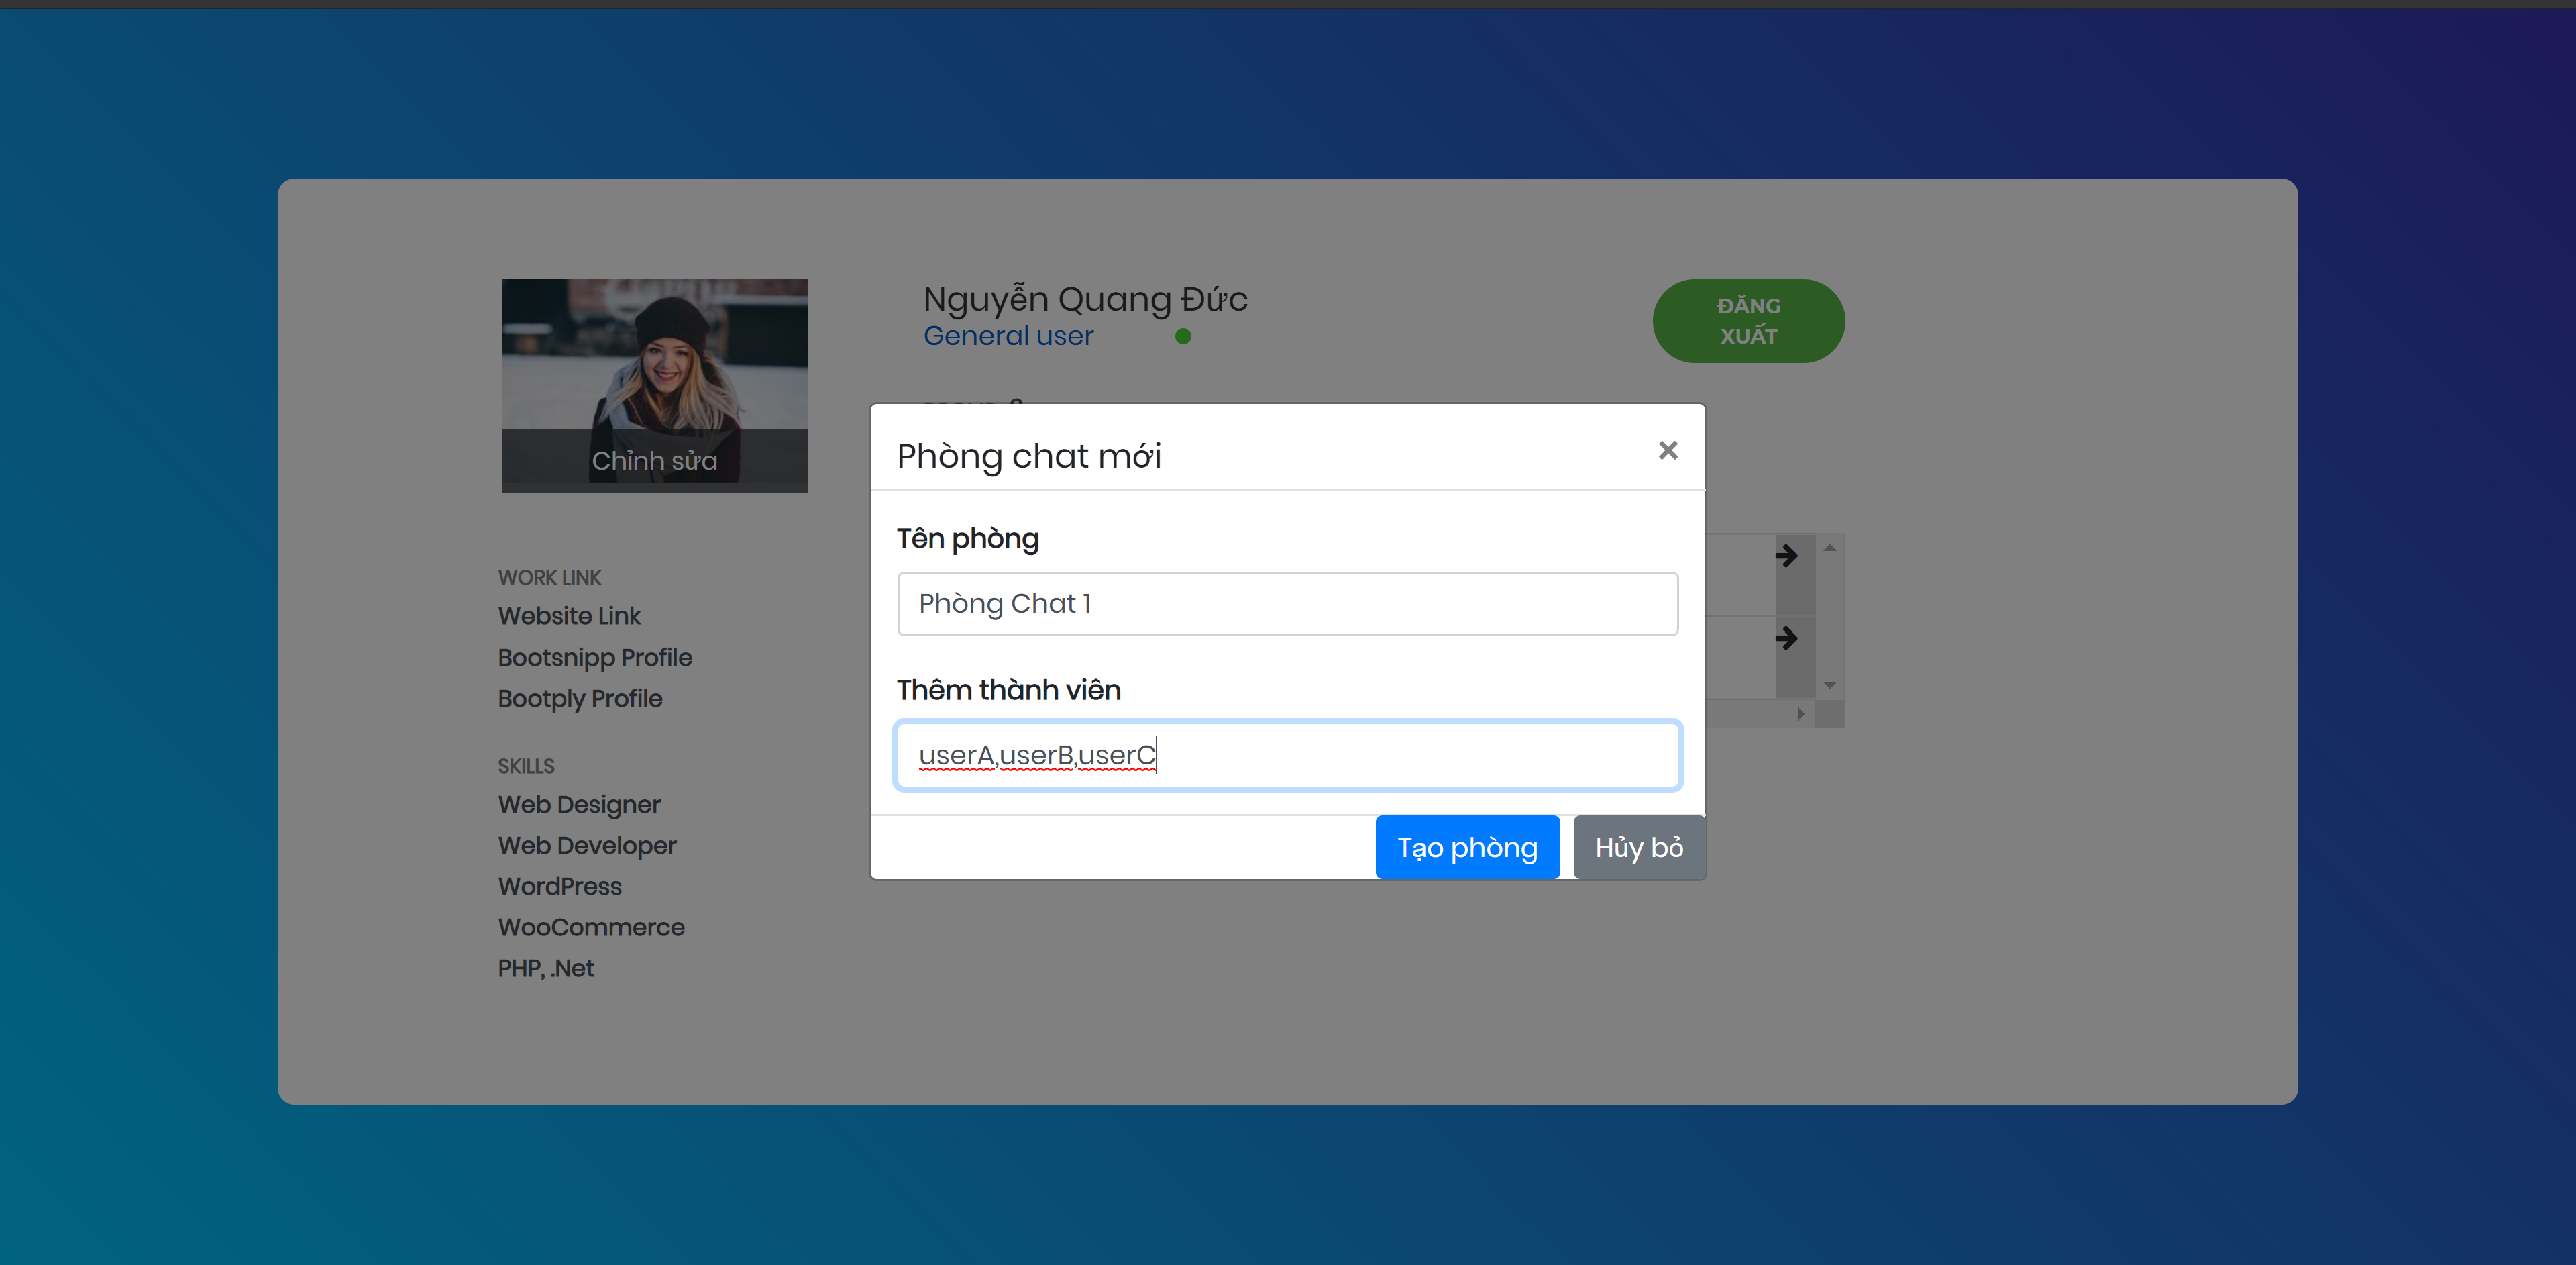
\includegraphics[scale=0.36]{add_user.png}
		\caption{Thêm bạn bè vào phòng chat}
		\label{F:add_user}
	\end{figure}
	
	\subsection{Vào phòng chat}
	Để vào phòng chat, người dùng chọn thẻ "Nhóm chat" trên trang cá nhân, sau đó chọn phòng chat muốn vào.
	
	\begin{figure}[H]
		\centering
		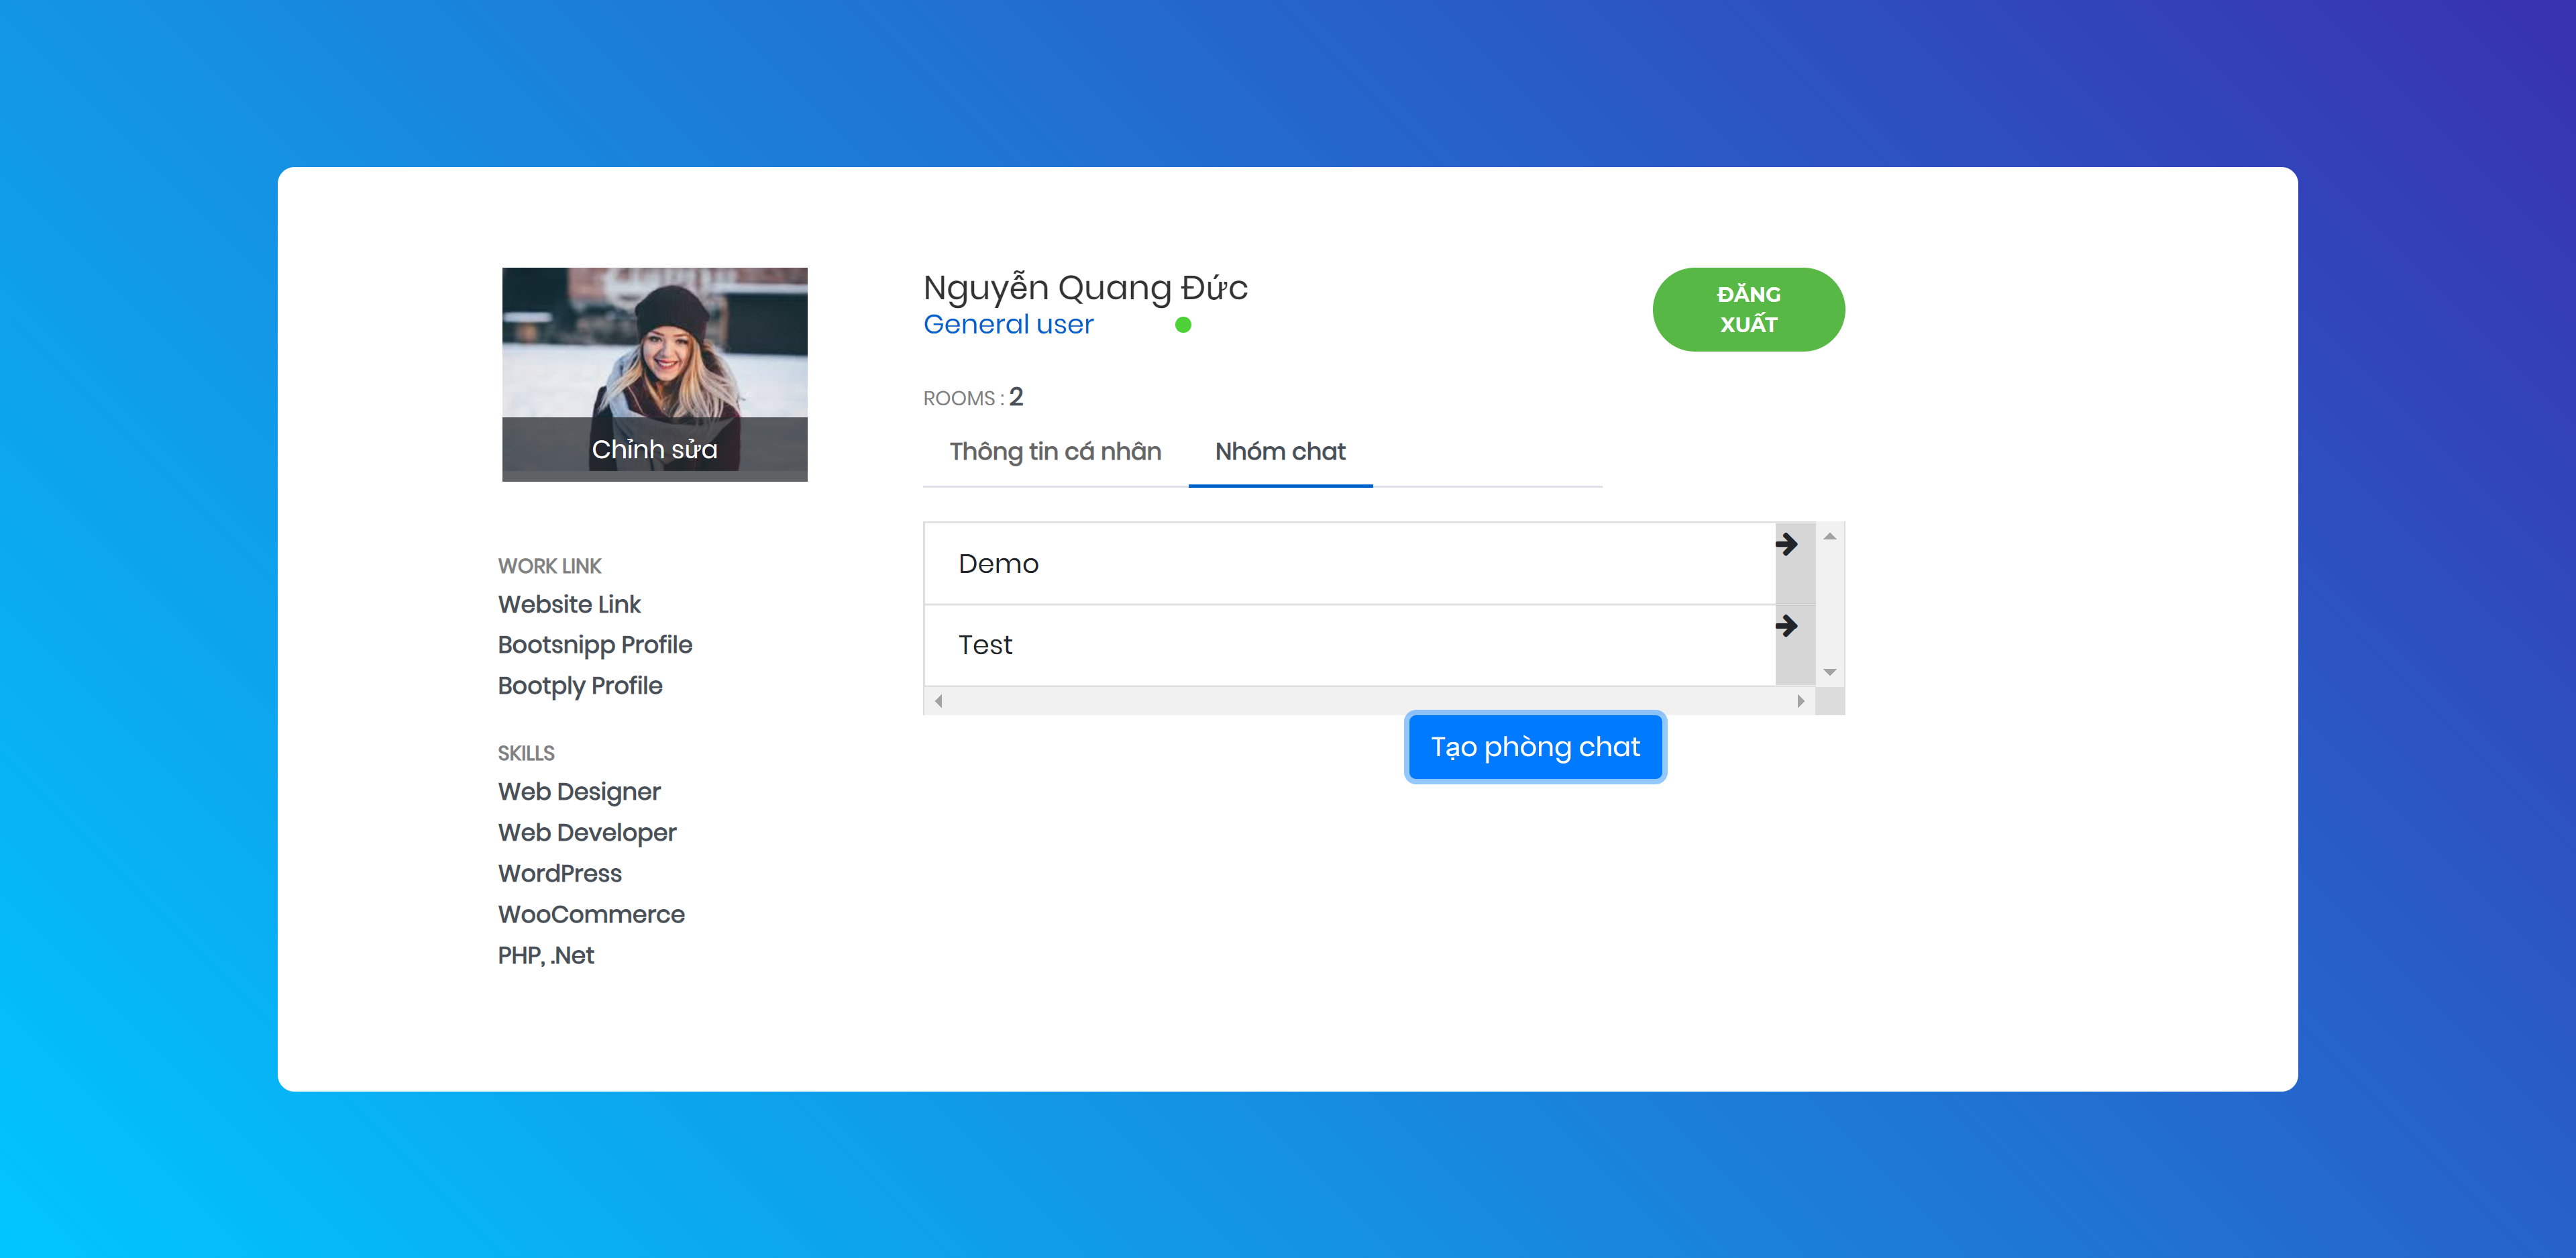
\includegraphics[scale=0.36]{view_room.png}
		\caption{Bấm vào phòng chat muốn vào}
		\label{F:view_room}
	\end{figure}
	
	\subsection{Gửi và nhận tin nhắn}
	Tại giao diện phòng chat, nhập tin nhắn cần gửi vào ô "Nhập tin nhắn" và nhấn "Gửi"
	
	\begin{figure}[H]
		\centering
		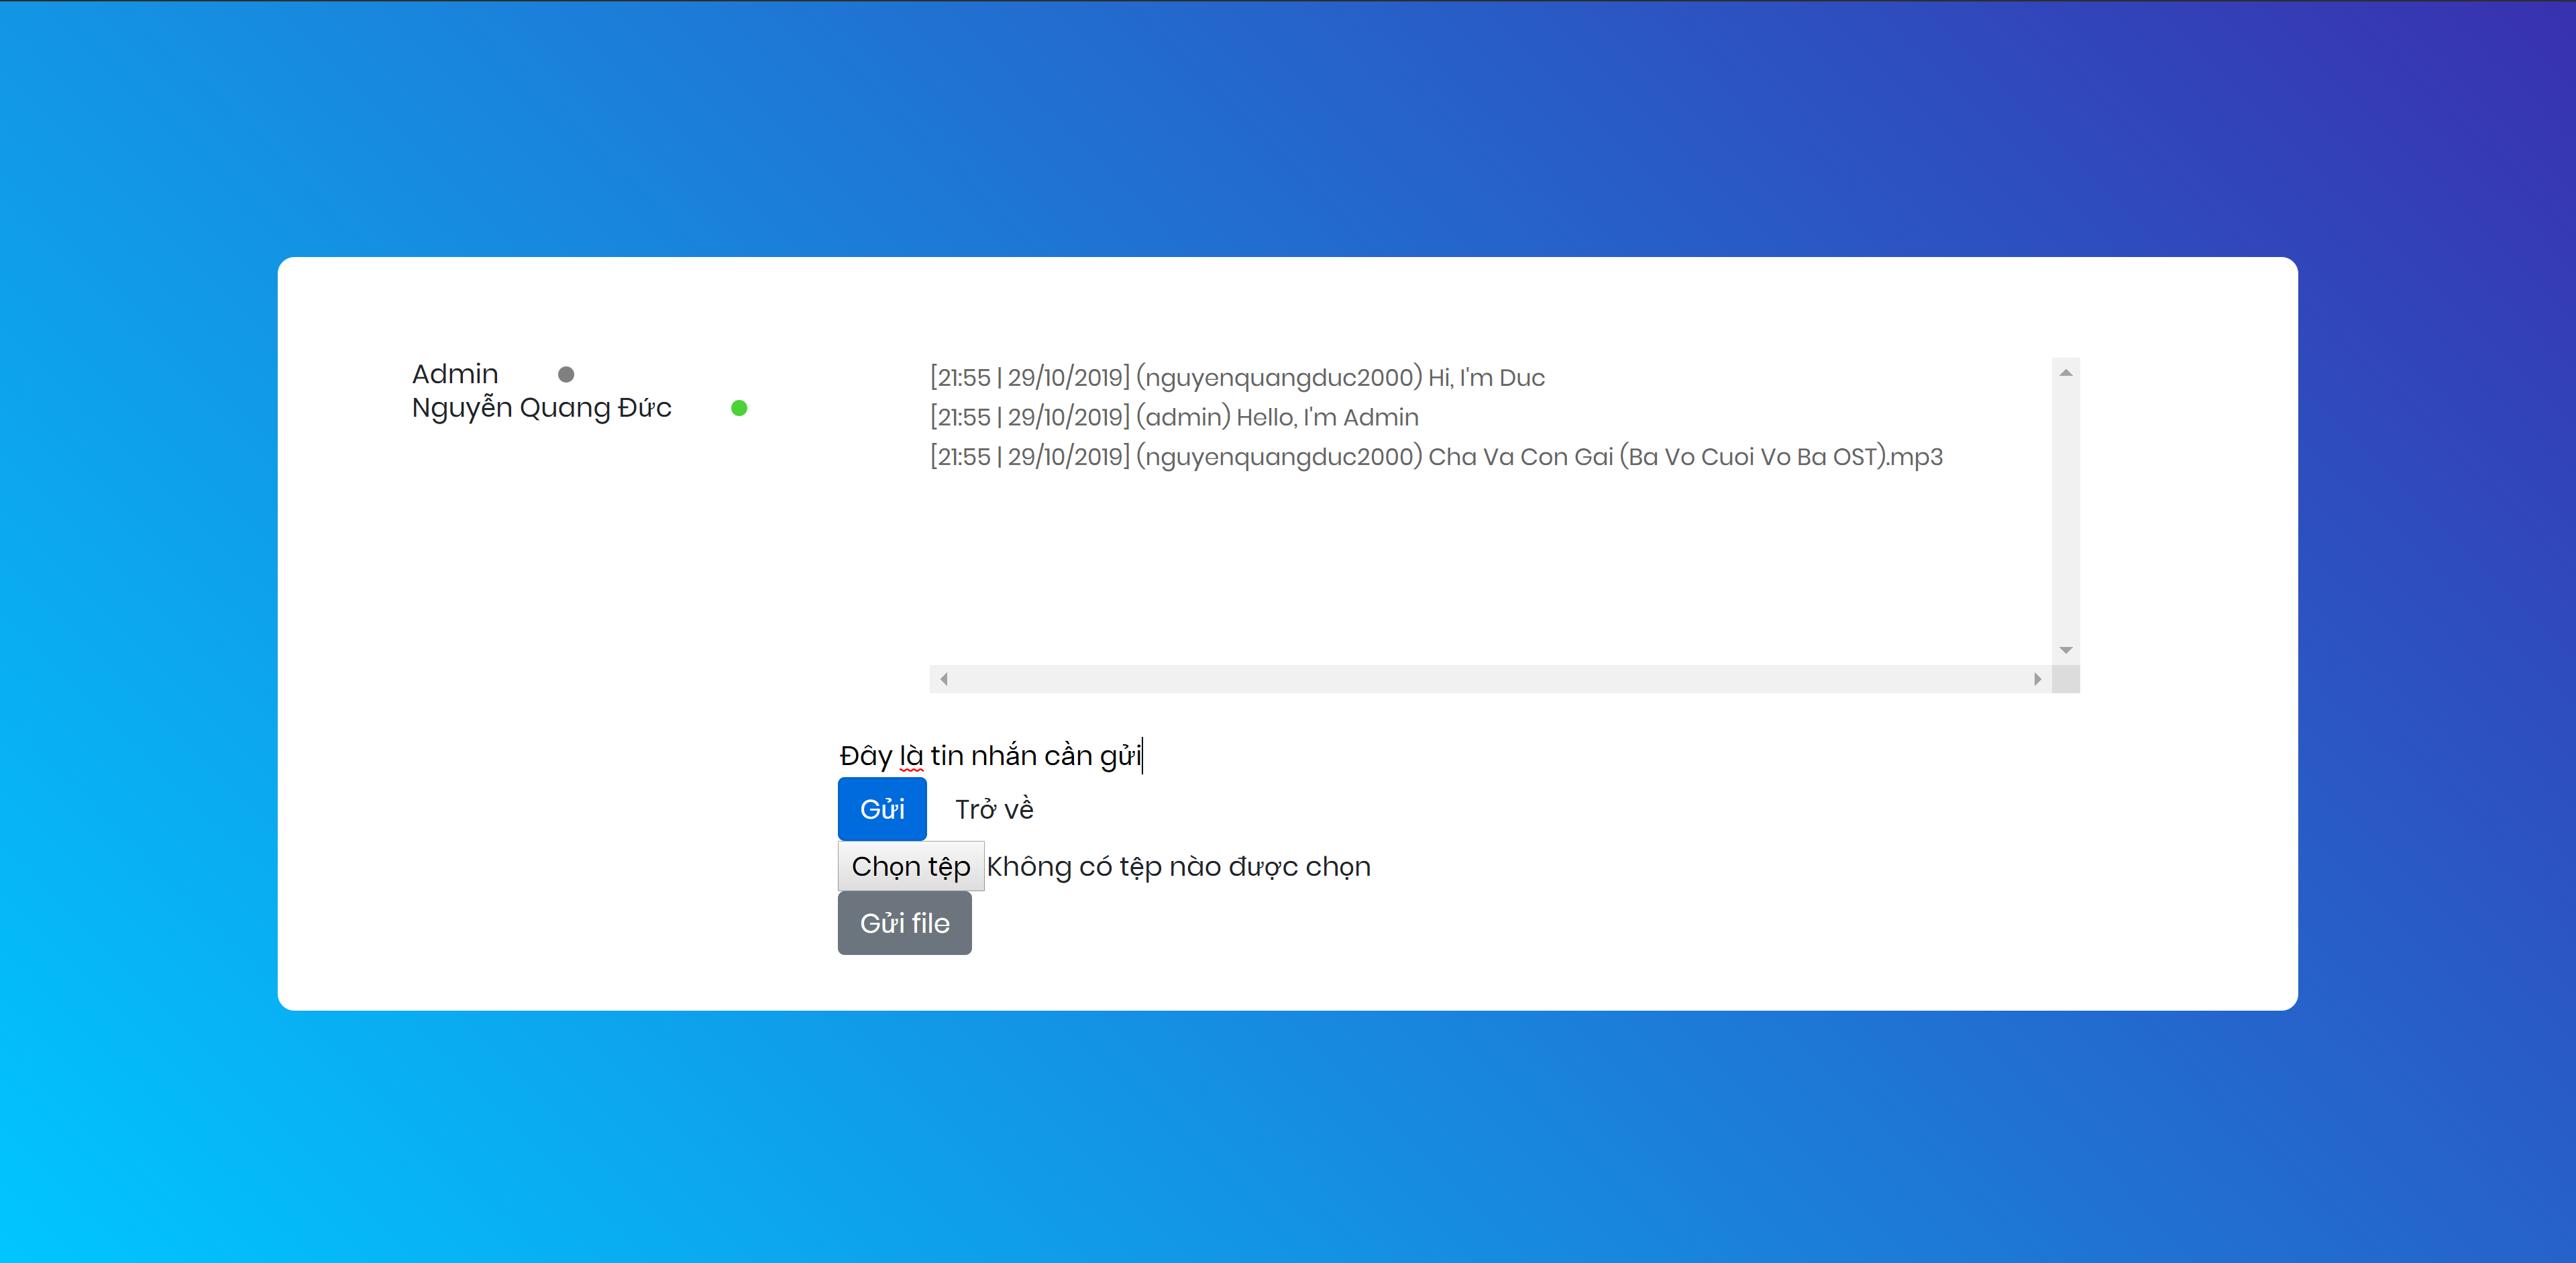
\includegraphics[scale=0.36]{send_message.png}
		\caption{Gửi tin nhắn}
		\label{F:send_message}
	\end{figure}
	
	\begin{figure}[H]
		\centering
		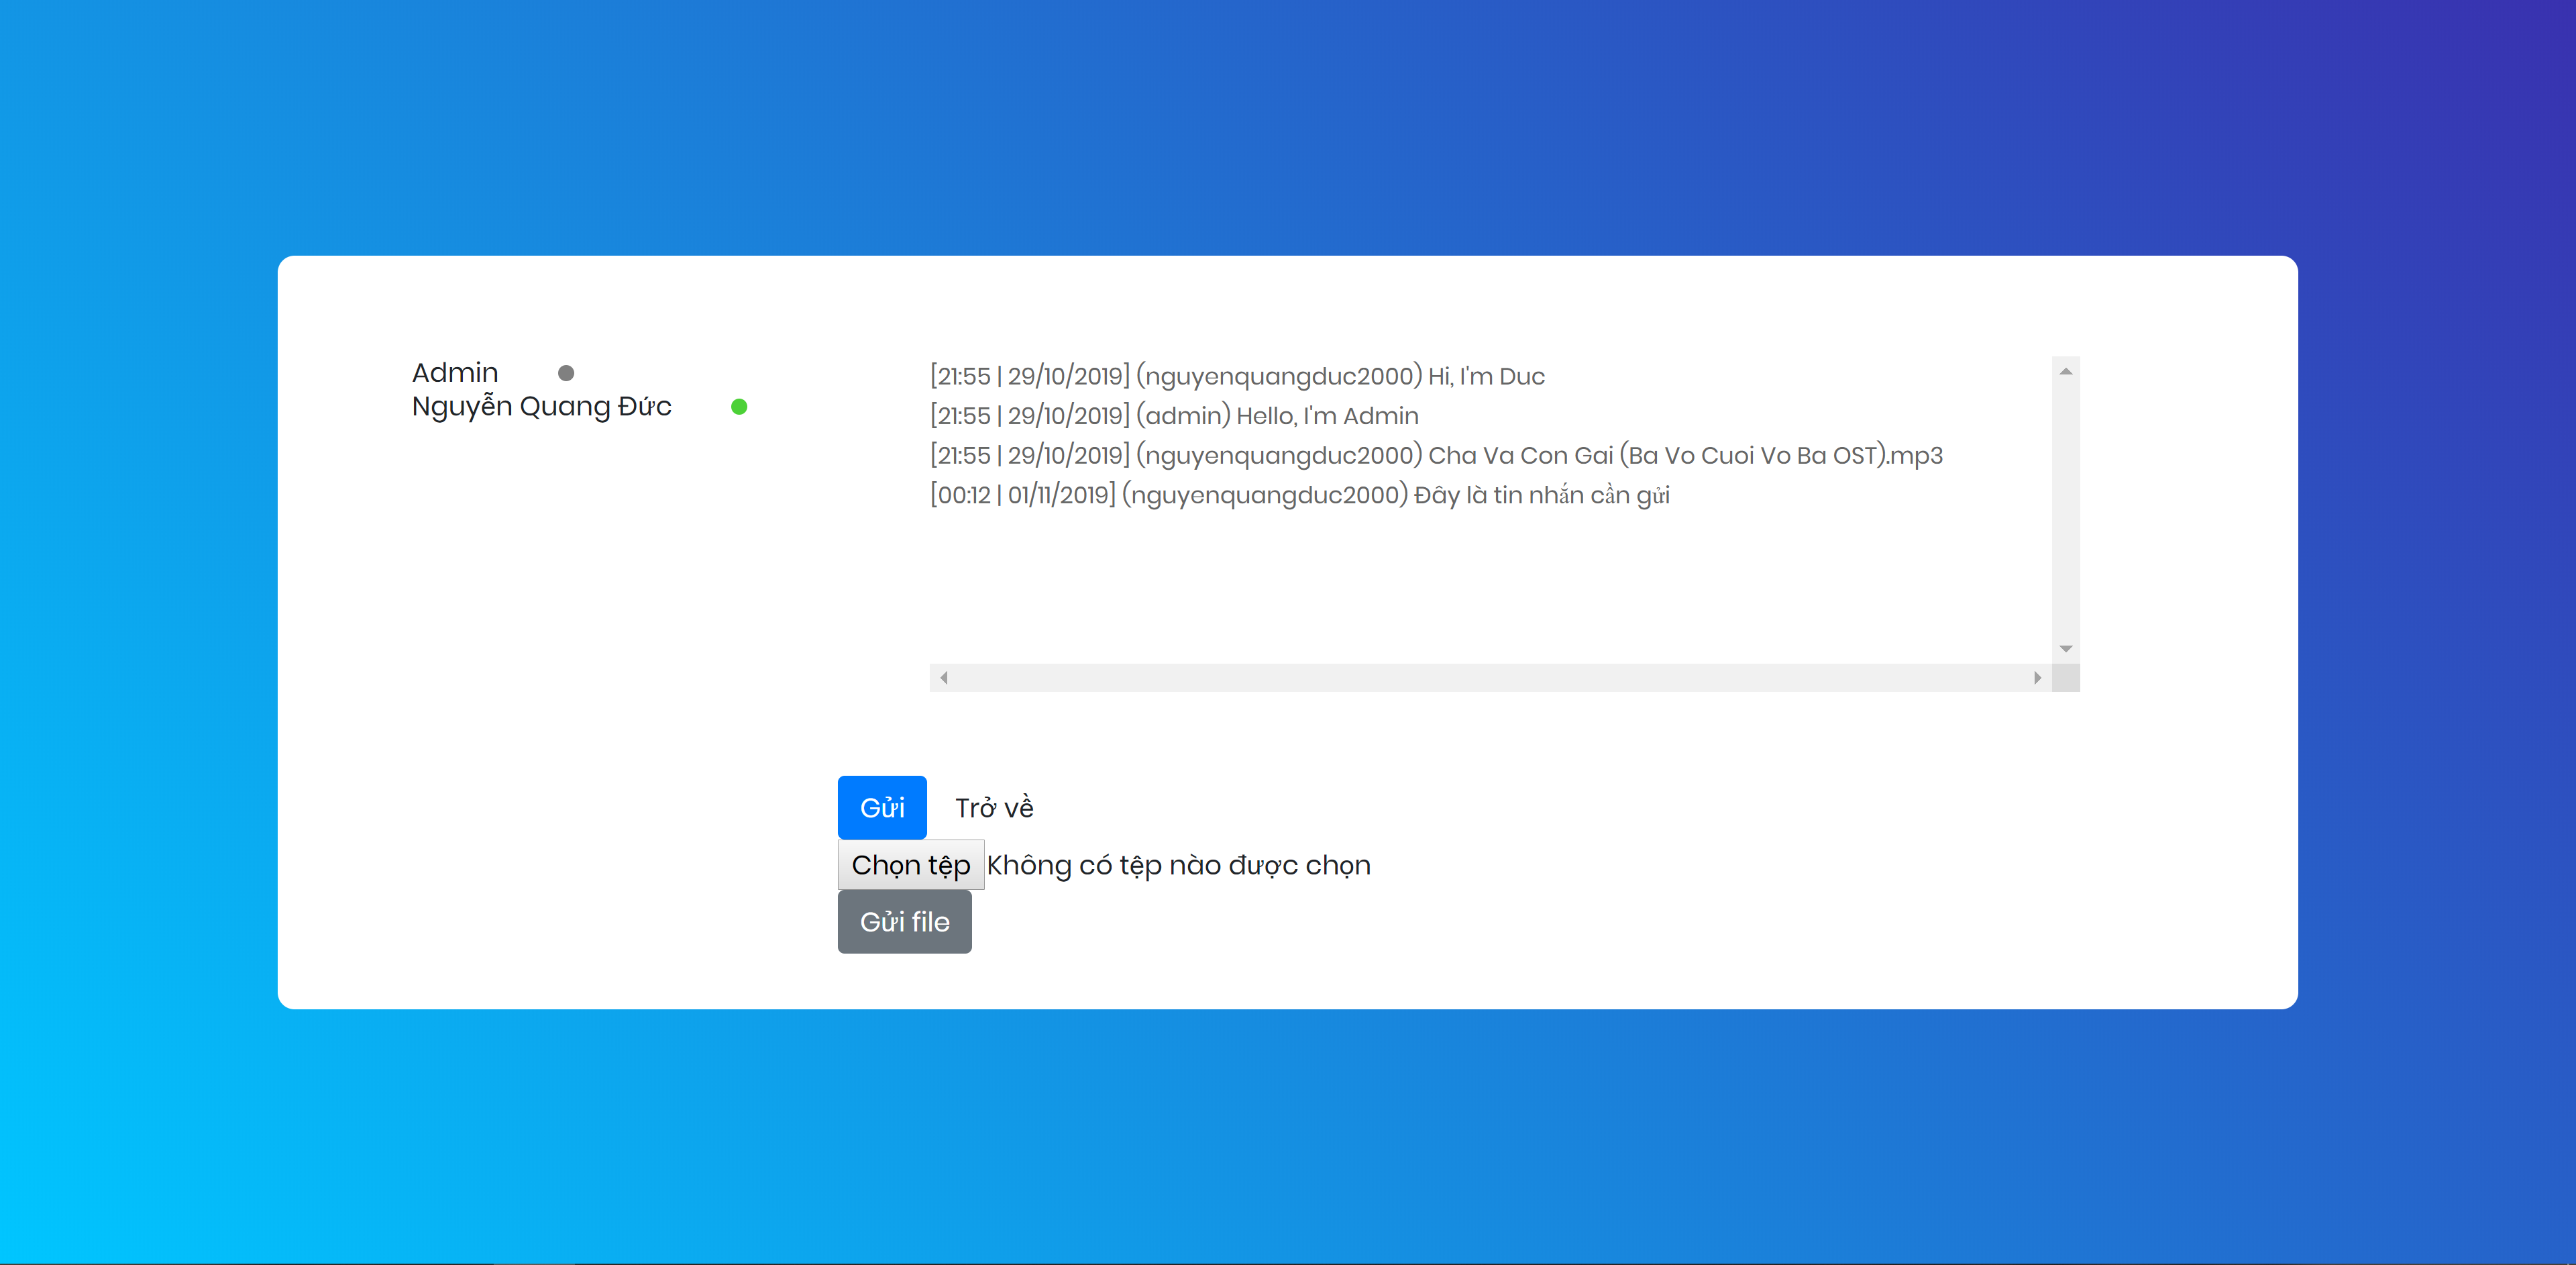
\includegraphics[scale=0.36]{send_message_success.png}
		\caption{Tin nhắn đã gửi thành công}
		\label{F:send_message_success}
	\end{figure}
	
	\subsection{Gửi và nhận file}
	Để gửi file, tại giao diện phòng chat bấm "Chọn tệp". Chọn file muốn gửi và bấm "Gửi file".\linebreak
	Để tải file, bấm vào tên file trên khung chat, file sẽ được tự động tải về.
	
	\begin{figure}[H]
		\centering
		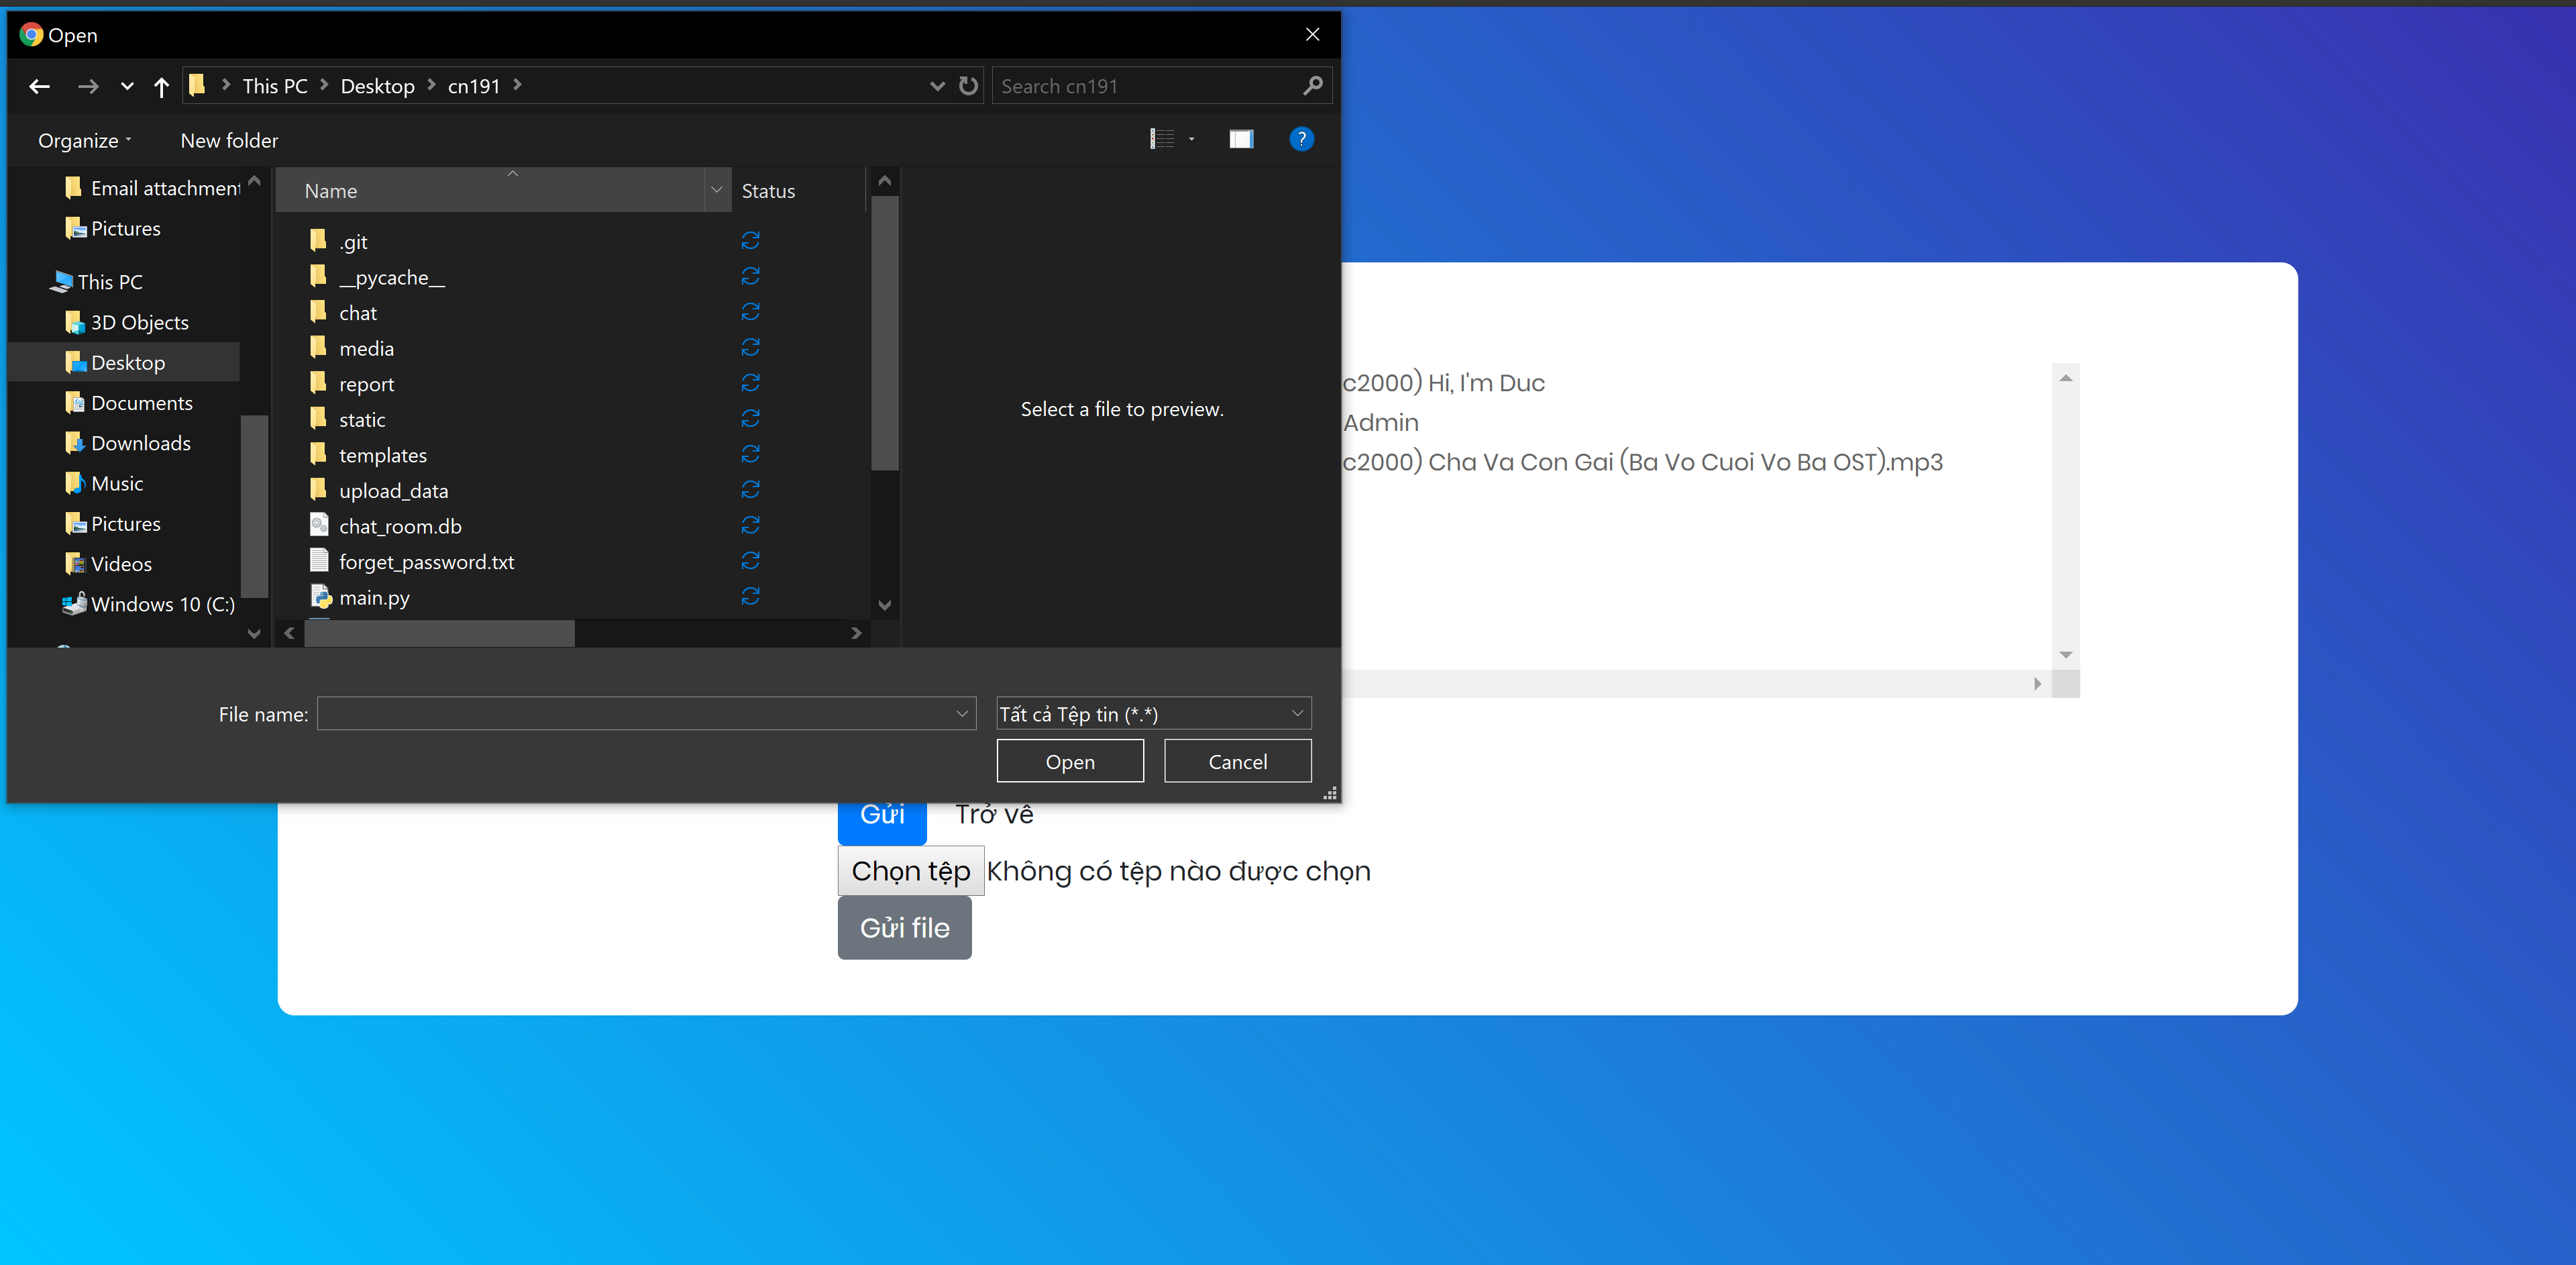
\includegraphics[scale=0.36]{send_file.png}
		\caption{Chọn file để gửi}
		\label{F:send_file}
	\end{figure}
	
	\begin{figure}[H]
		\centering
		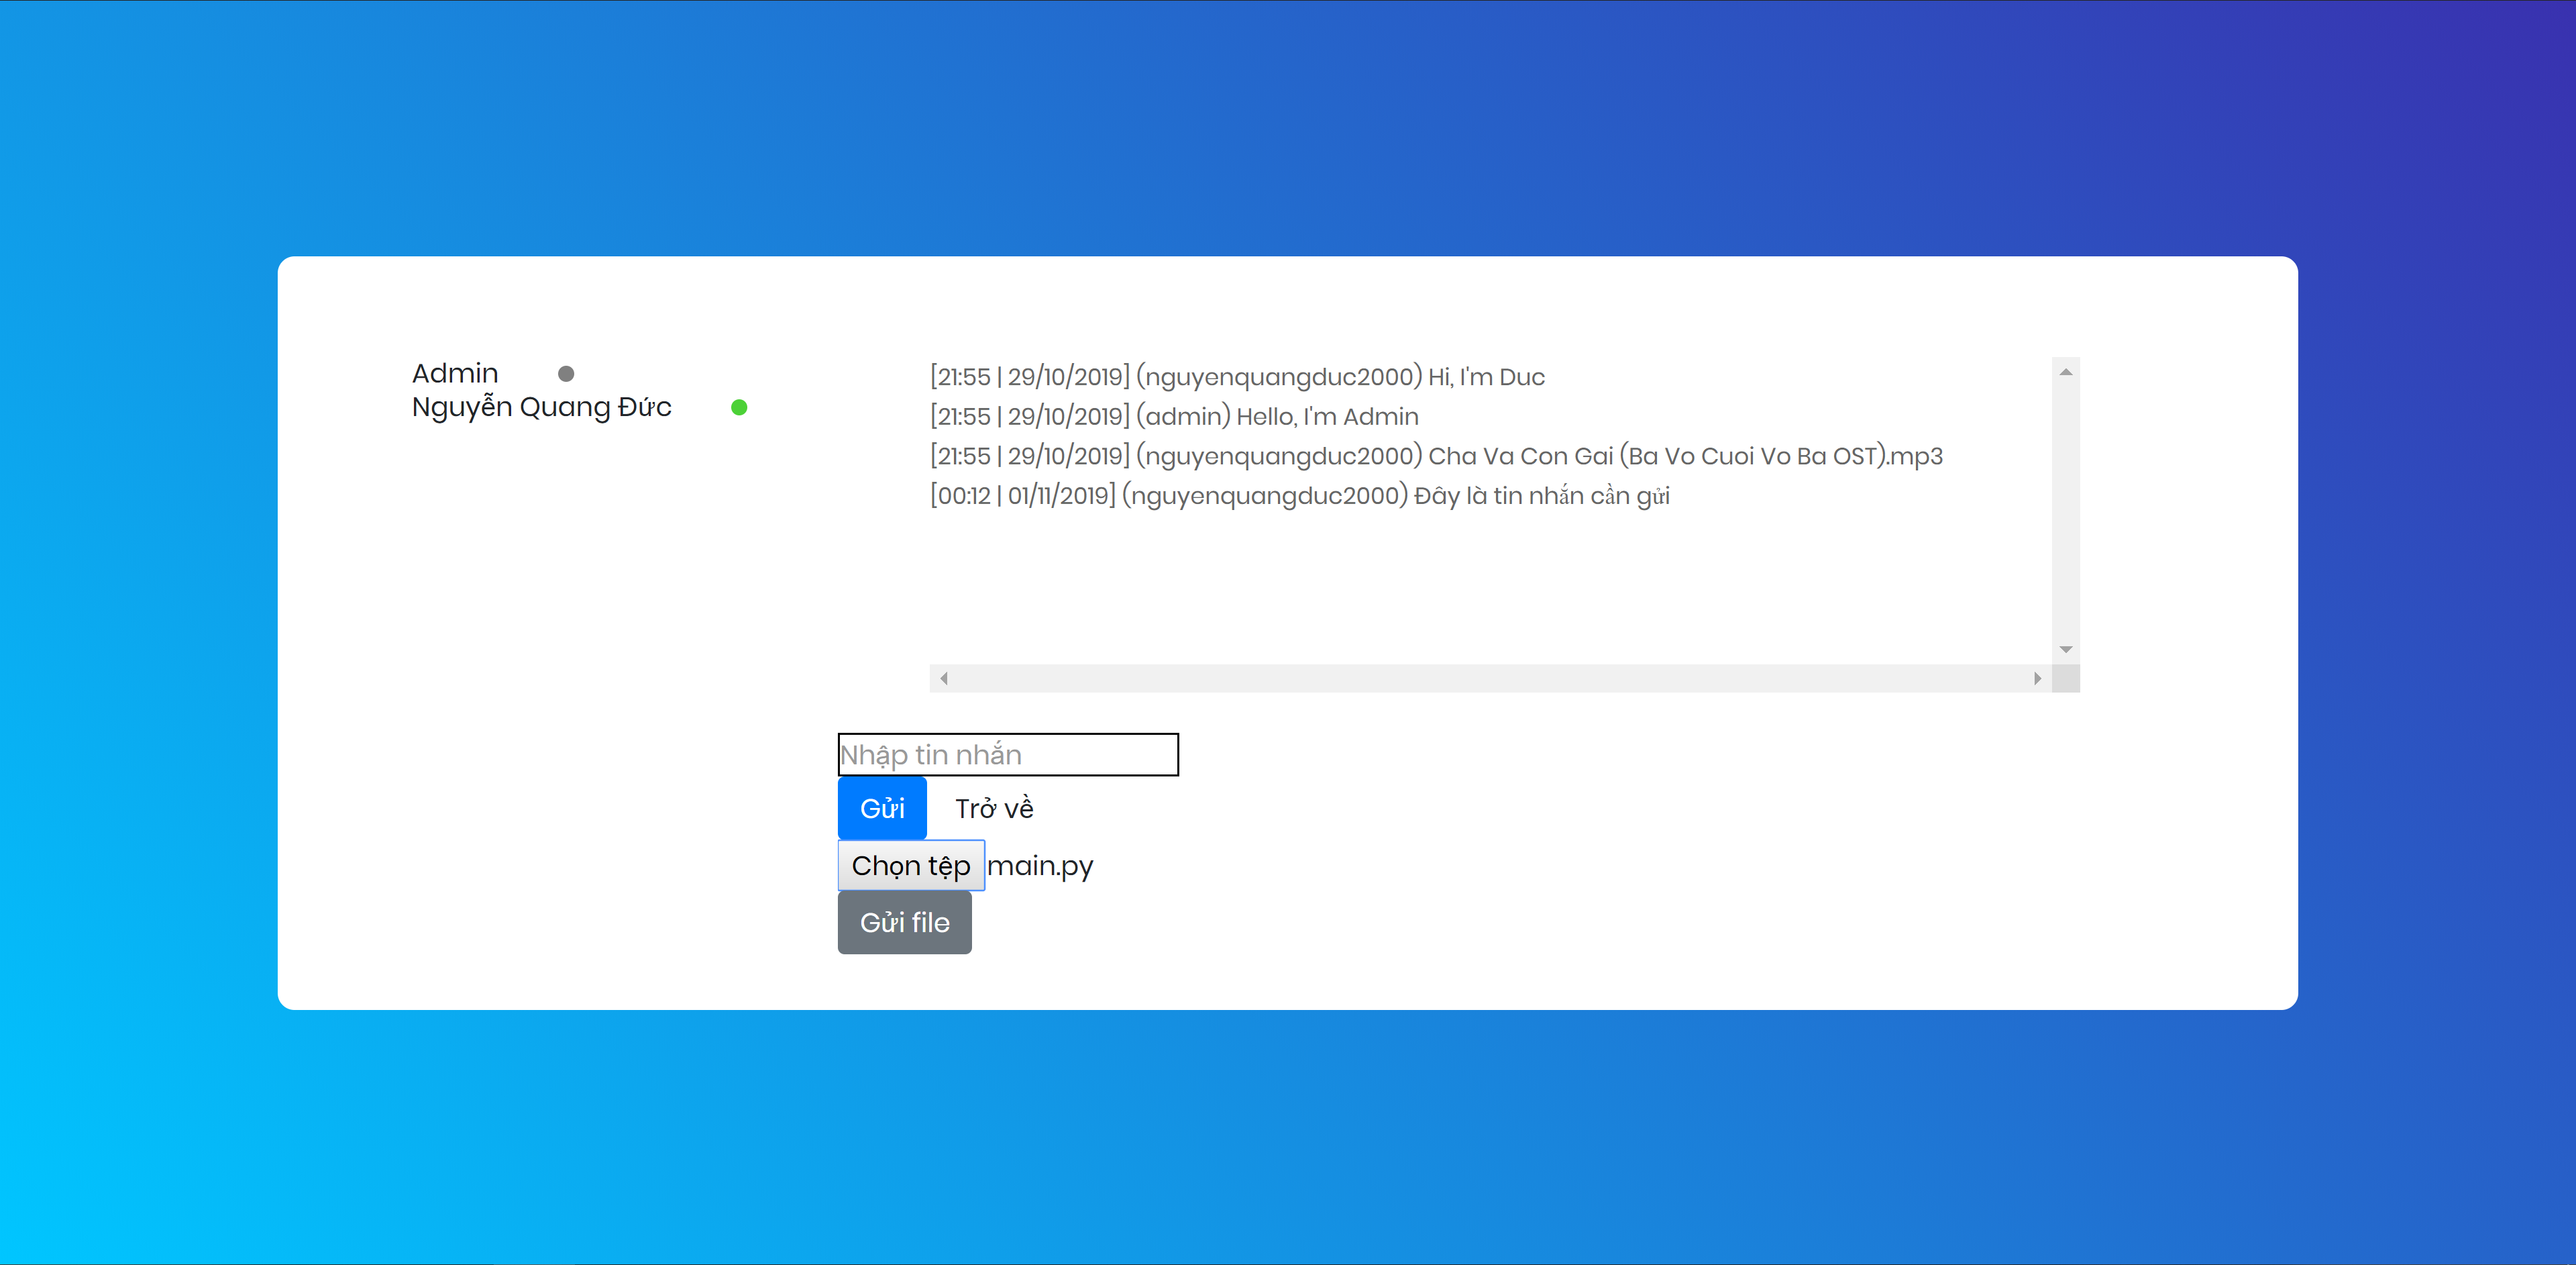
\includegraphics[scale=0.36]{send_file_prepare.png}
		\caption{File đã sẵn sàng để gửi}
		\label{F:send_file_prepare}
	\end{figure}
	
	\begin{figure}[H]
		\centering
		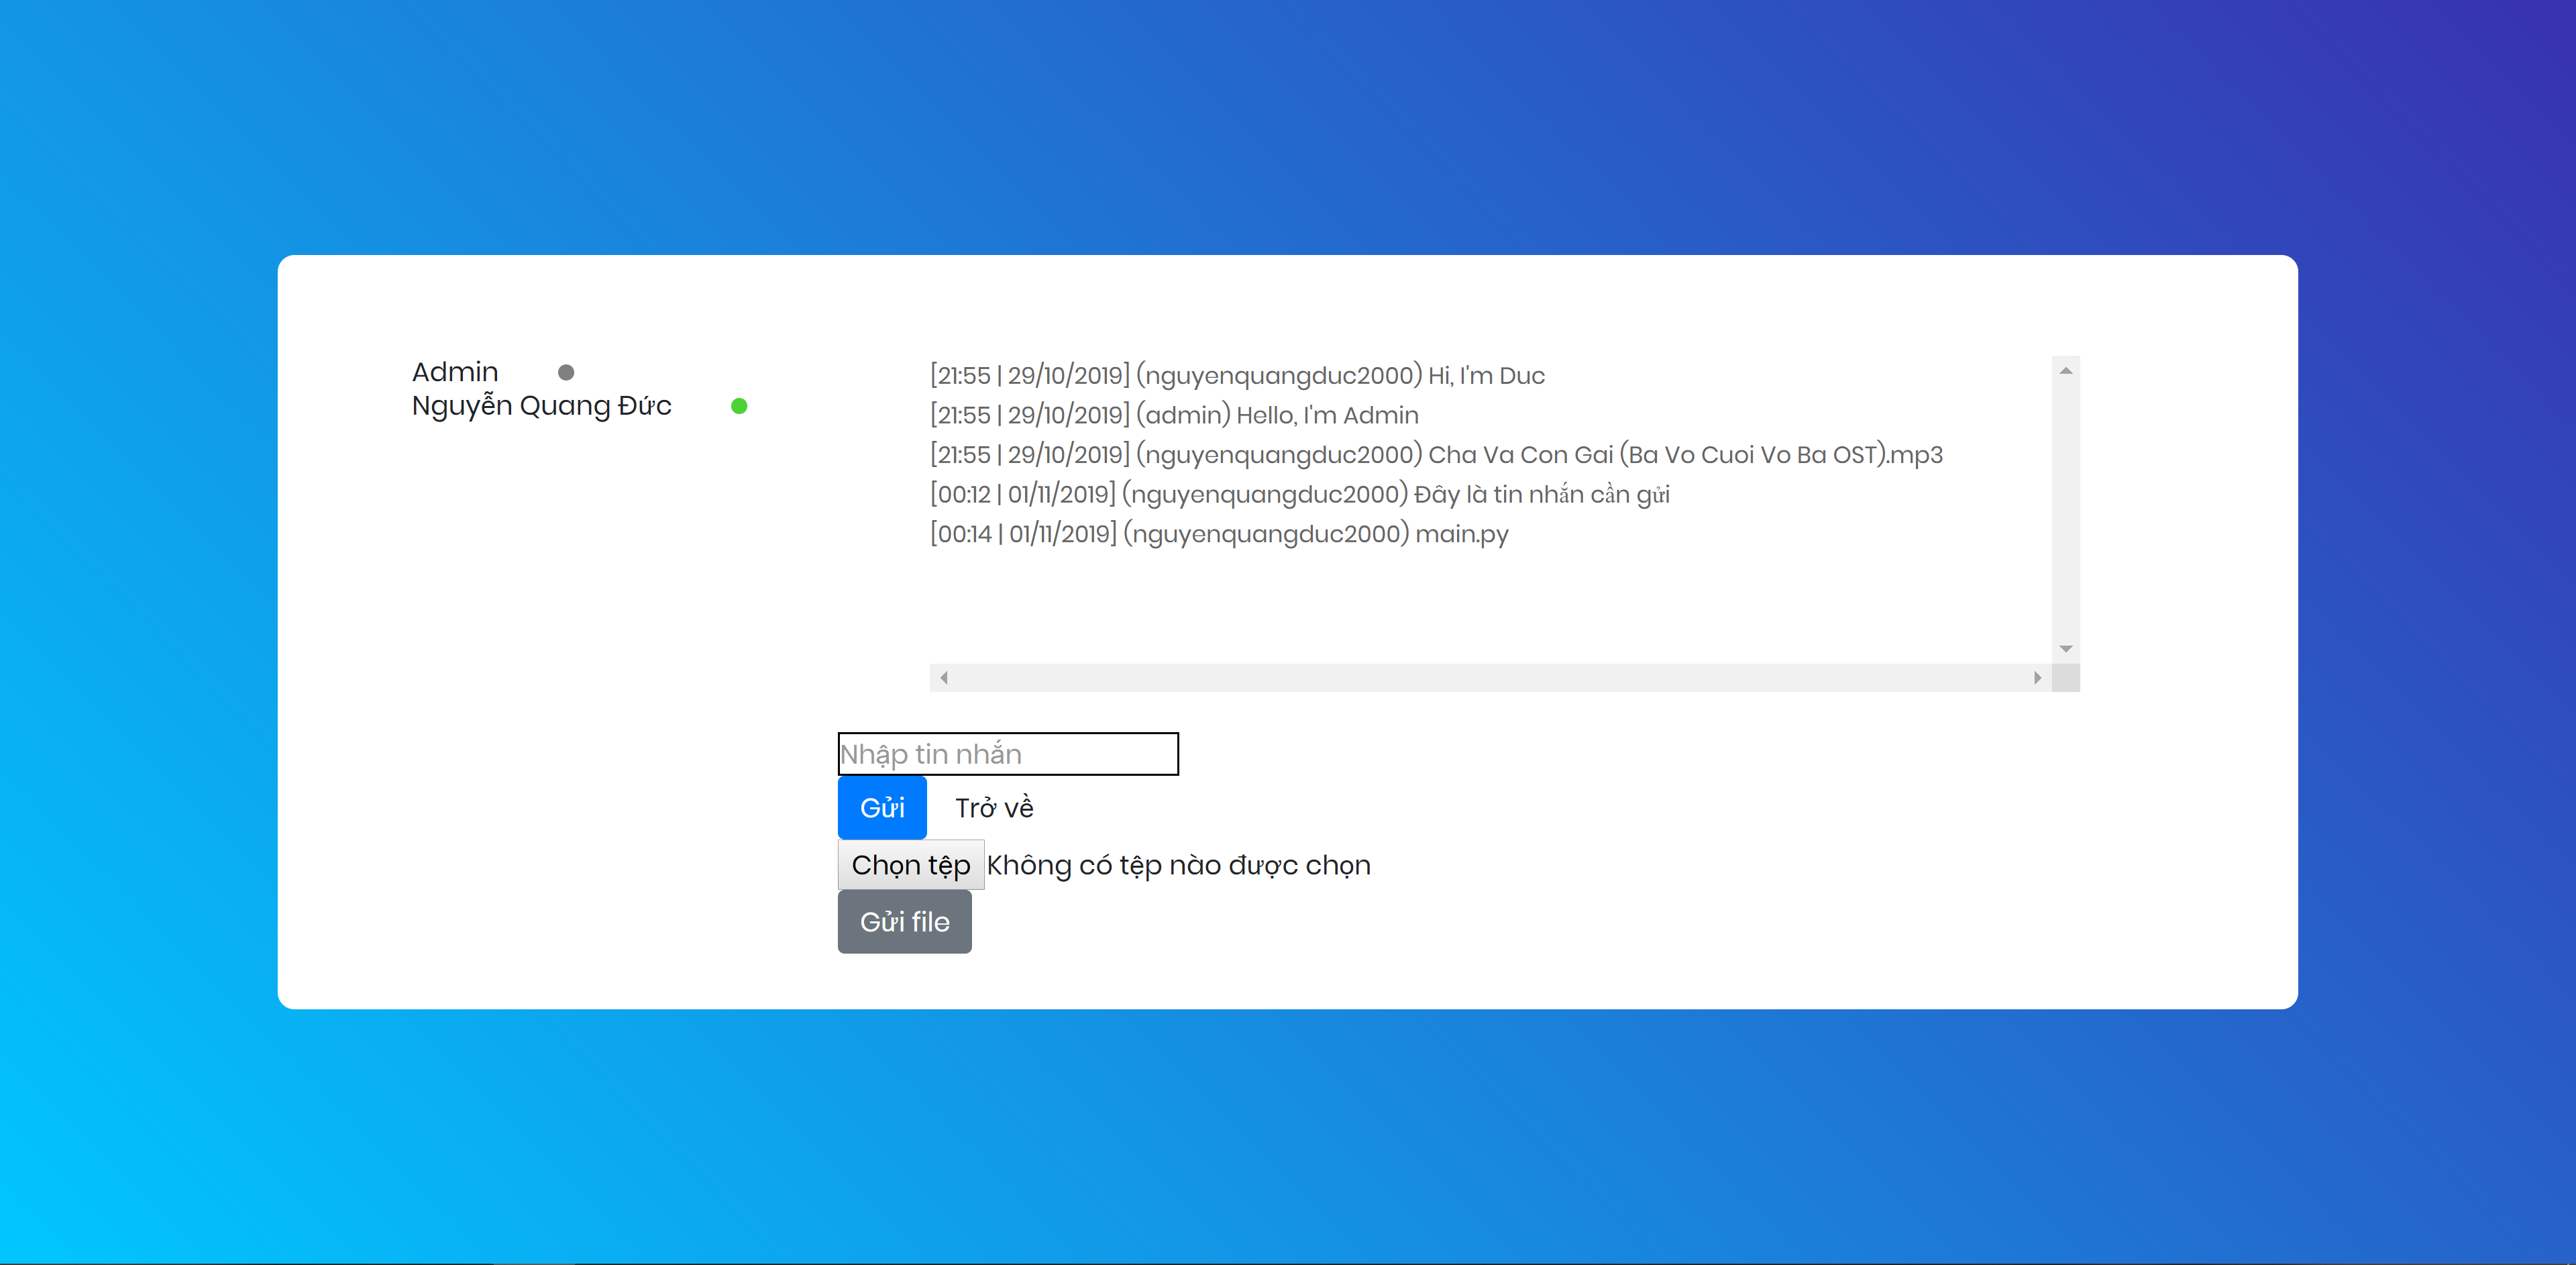
\includegraphics[scale=0.36]{send_file_success.png}
		\caption{Gửi file thành công}
		\label{F:send_file_success}
	\end{figure}
	
	\subsection{Xem trạng thái của thành viên khác}
	Thông tin của các thành viên trong phòng chat luôn nằm ở góc trên bên trái màn hình. Tại đây, nếu thành viên phòng chat đang online sẽ có chấm xanh sáng, ngược lại chấm xanh sẽ tắt.
	
	\begin{figure}[H]
		\centering
		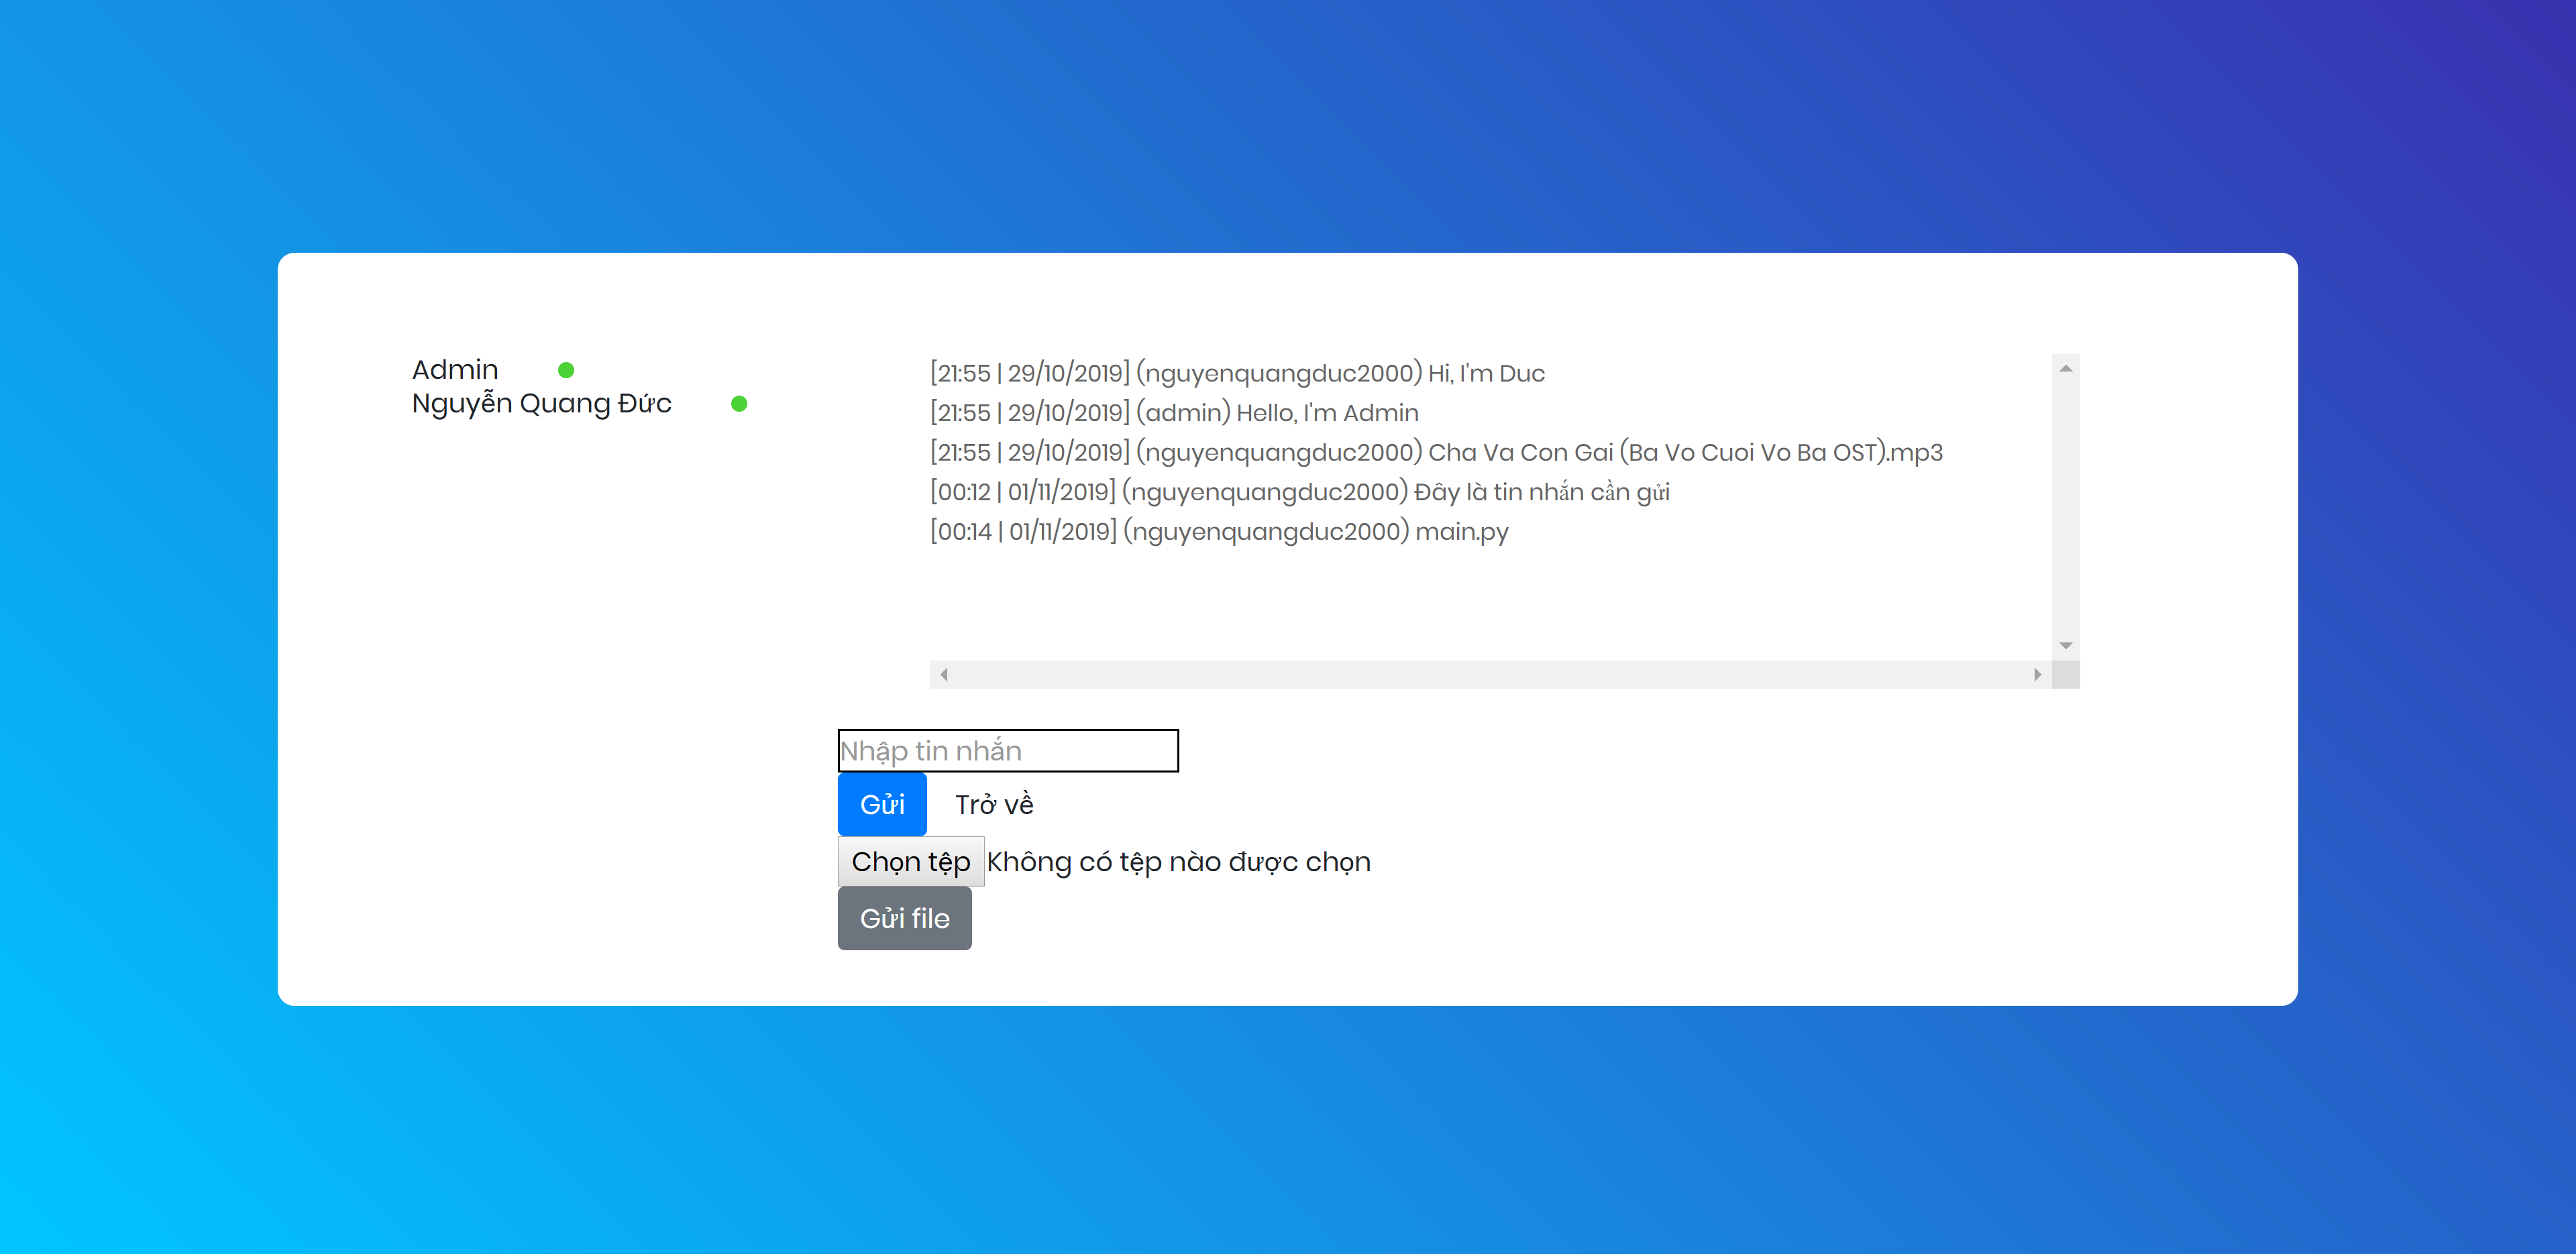
\includegraphics[scale=0.36]{user_status_online.png}
		\caption{Người dùng "Admin" đang online}
		\label{F:user_status_online}
	\end{figure}
	
	\begin{figure}[H]
		\centering
		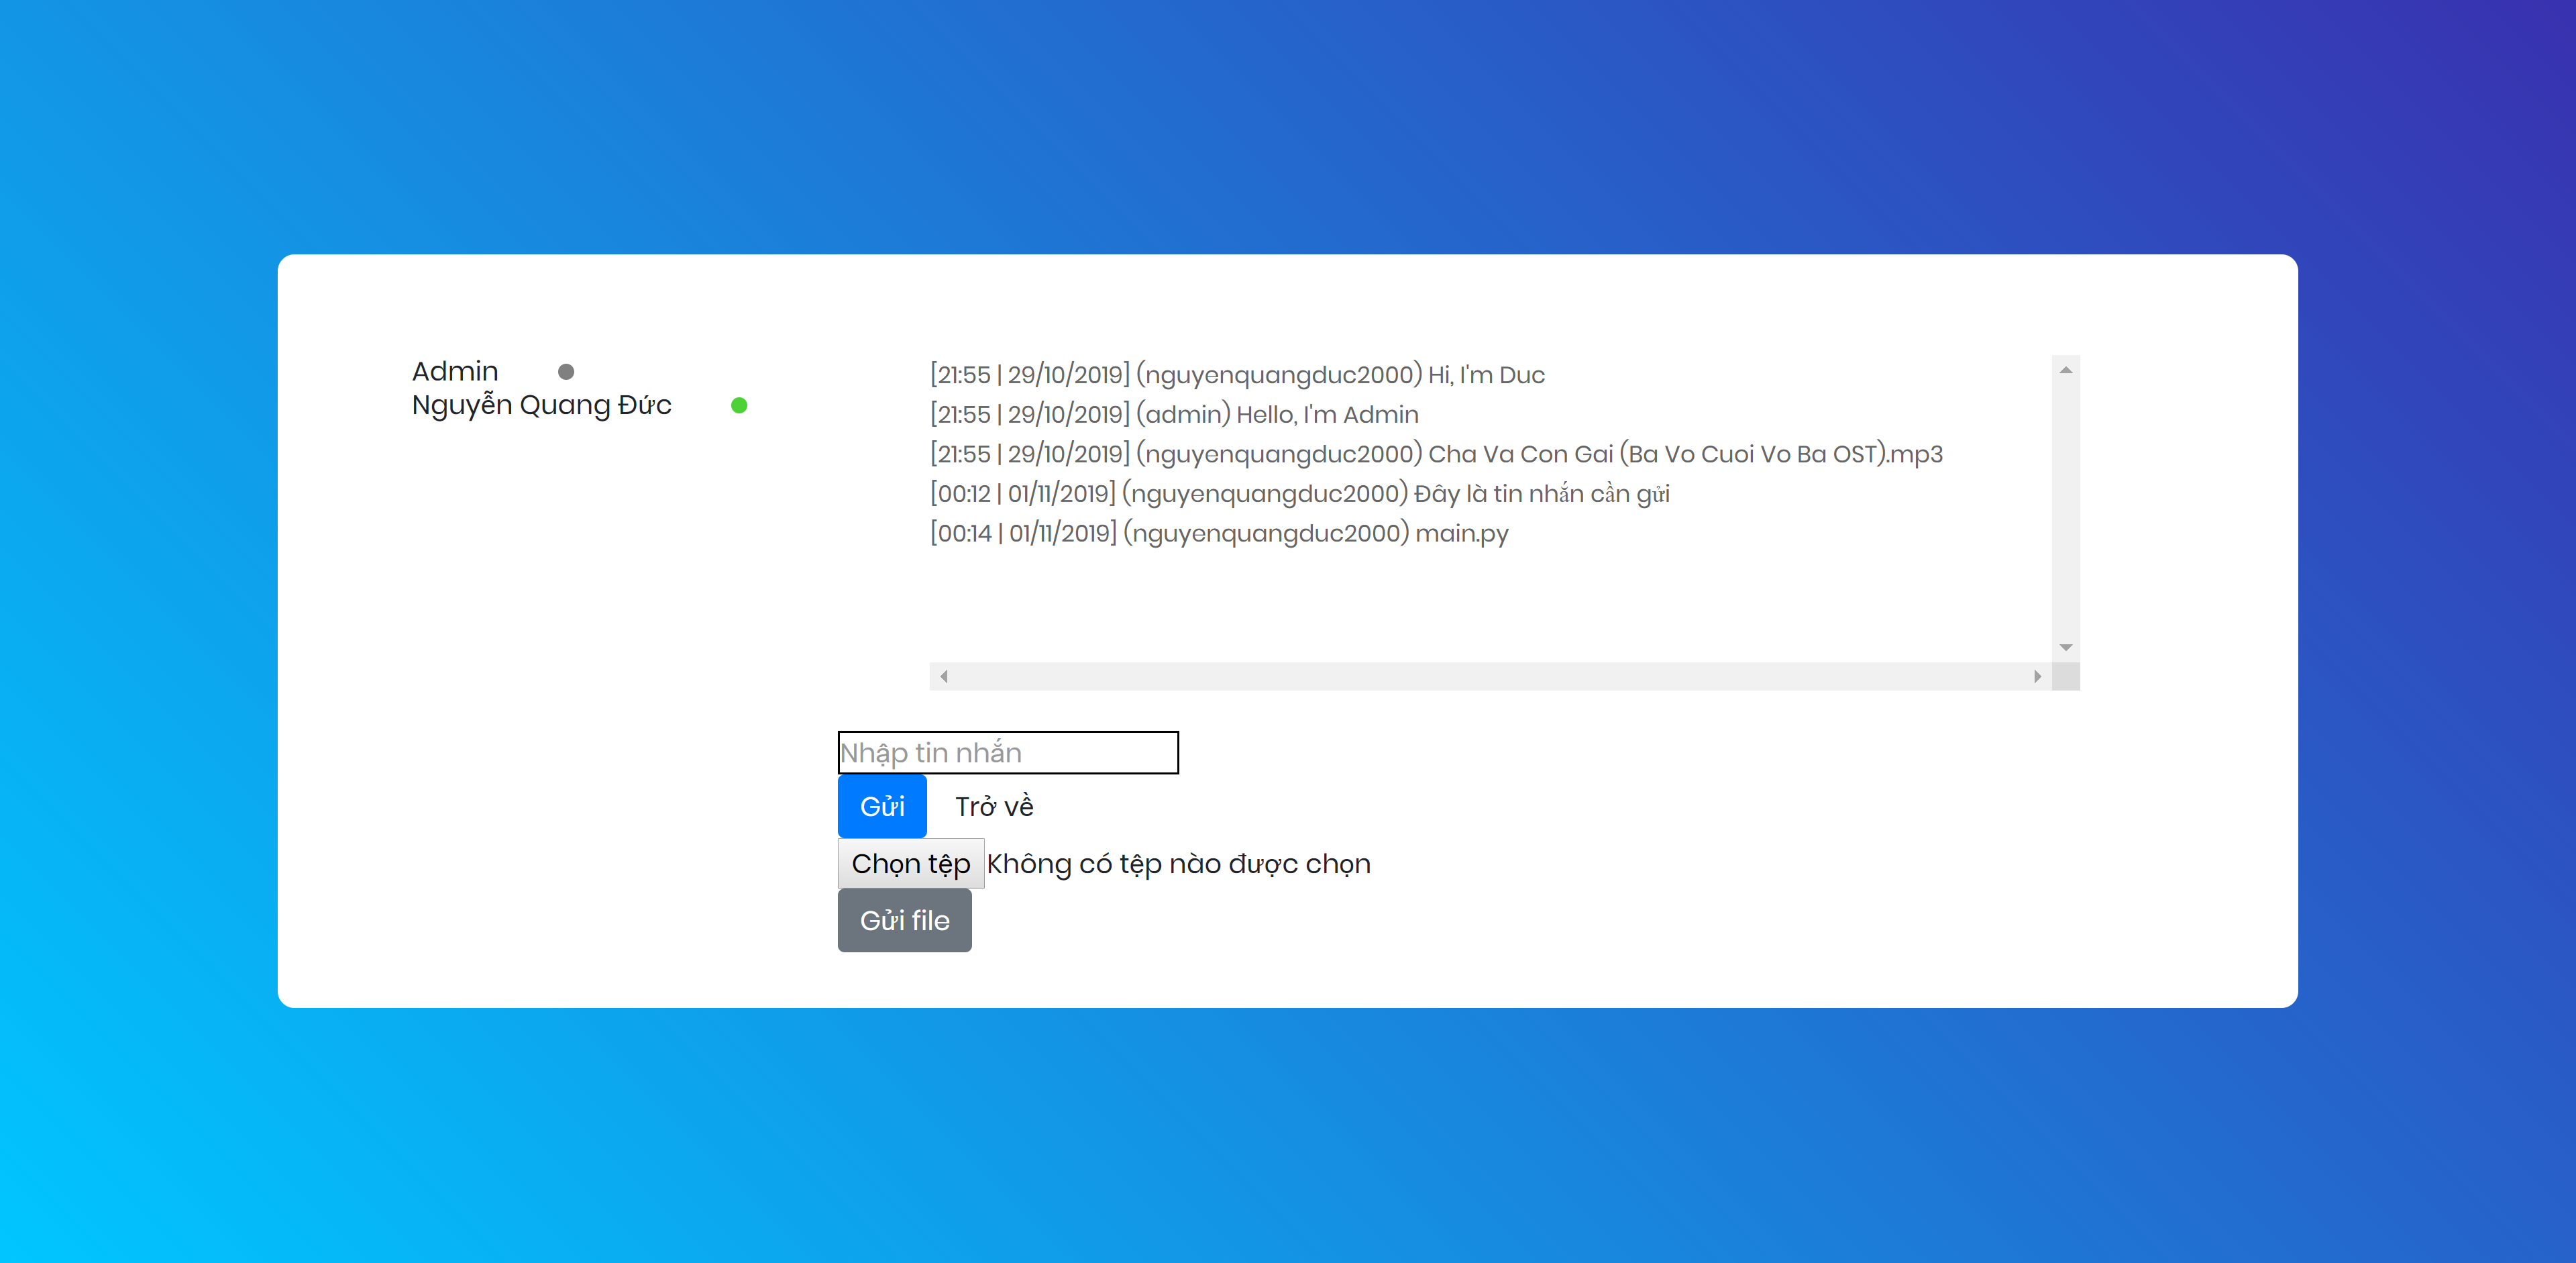
\includegraphics[scale=0.36]{user_status_offline.png}
		\caption{Người dùng "Admin" đang offline}
		\label{F:user_status_offline}
	\end{figure}
	

\end{document}

